\documentclass[a4paper,12pt]{book}
\usepackage{graphicx}
\usepackage[export]{adjustbox}
\usepackage{subcaption}
\graphicspath{{Pics/}}
\usepackage{charter}
\usepackage{fancyhdr}
\usepackage{enumerate}
\usepackage{enumitem}
\usepackage{siunitx}
\usepackage{amssymb}
\usepackage{longtable}
\usepackage{multicol}
\usepackage{multirow}
\usepackage{hhline}
\usepackage{parskip}
\setlength{\parskip}{6pt}
\usepackage{ragged2e}
\usepackage{geometry} %margin
\geometry{left=2.1cm,right=2.1cm,top=3cm,bottom=3cm}
\usepackage{setspace}
\SetSinglespace{1.2}
\singlespacing
\renewcommand{\ttfamily}{\fontfamily{pcr}\selectfont}
%\renewcommand{\familydefault}{\rmdefault}

\usepackage[,table]{xcolor}
\definecolor{LightBlue}{cmyk}{0.16,0.03,0.04,0}
\definecolor{Title}{cmyk}{0.8,0.1,0,0.3}
\setlength{\arrayrulewidth}{0.3mm}
\setlength{\tabcolsep}{2pt}
\setlength{\headheight}{15pt}
\renewcommand{\arraystretch}{1}
\usepackage{tikz}
\usepackage{nicematrix}
\newcommand*\circled[1]{\tikz[baseline=(char.base)]{\node[shape=circle,draw,inner sep=1pt] (char) {#1};}}

\newcolumntype{s}{>{\columncolor{Title}\RaggedLeft} m{3.5em}} % columntype for chapter title
\newcolumntype{d}{>{\columncolor{LightBlue}\RaggedRight} m{\textwidth}} % columntype for code bloc
\newcolumntype{a}{>{\columncolor{LightBlue}\RaggedRight} m{0.96\textwidth}} % columntype for secondary code bloc

\usepackage{titlesec}
\usepackage[hidelinks]{hyperref}
\urlstyle{same}

\captionsetup[figure]{labelsep=period,font={bf}}
\captionsetup[table]{font={bf},labelsep=period}

\newcommand{\titlename}{}

\newcommand{\chaptertitle}[2]{ %reset chapter format
\vspace{-120pt}
\gdef\titlename{#1}
{
\SetSinglespace{1.1}
\singlespacing
\Huge\bfseries
\setlength{\tabcolsep}{8pt}
\renewcommand{\arraystretch}{1.5}
\begin{tabular}{s >{\RaggedRight}m{14.5em}}
\textcolor{white}{Chapter\newline\thechapter}&\textcolor{Title}{#2}
\end{tabular}
}
}

\newcommand{\partpic}[1]{%insert picture
    \tikz[remember picture,overlay] \node at (current page.center){\includegraphics[width=\paperwidth]{#1}};
}

\titleformat{\part} %reset part %format
{\huge\bfseries} % format
{} % label
{0em} % sep
{\Centering} % before-code

\titleformat{\chapter} %reset chapter %format
{\huge\bfseries} % format
{} % label
{0em} % sep
{\Centering} % before-code
\titlespacing{\chapter}{0pt}{0pt}{0pt}

\titleformat{\section} %reset section %format
{\Large\bfseries} % format
{\textcolor{Title}{\thesection}} % label
{0.5em} % sep
{\color{Title}} % before-code
\titlespacing{\section}{0pt}{12pt}{6pt}

\titleformat{\subsection} %reset subsection %format
{\large\bfseries} % format
{\textcolor{Title}{\thesubsection}} % label
{0.5em} % sep
{\color{Title}} % before-code
\titlespacing{\subsection}{0pt}{8pt}{6pt}

\newenvironment{term}[1]{
    \textbf{#1}

    \leftskip 1em
    \parskip 0pt
}

\newenvironment{secterm}[1]{
    \textbf{#1}

    \leftskip 2em
    \parskip 0pt
}

\newenvironment{codebloc}{ %define code bloc style
    \ttfamily\footnotesize
    \renewcommand{\arraystretch}{1}
}

\newcommand{\note}[2][NOTE]{ %Note/Tips
\vspace{6pt}
\begin{tabular}{b{\textwidth}}
\hline
\fontfamily{phv}\selectfont \textbf{#1}\\
\leftskip 1em #2\\
\hline
\end{tabular}
}

\newcommand{\secnote}[2][NOTE]{ %Note/Tips
\vspace{6pt}
\begin{tabular}{b{0.93\textwidth}}
\hline
\fontfamily{phv}\selectfont \textbf{#1}\\
\leftskip 1em #2\\
\hline
\end{tabular}
}

\title{ESP32-C3 Wireless Adventure\par \Large A comprehensive guide to IoT}
\author{Espressif Systems}
\date{\today}

\pagestyle{fancy} % reset head&foot
\fancyhead{} % clear all header fields
\renewcommand\headrulewidth{0pt}
\fancyfoot{} % clear all footer fields
\setcounter{chapter}{8}

\begin{document}

\fancyfoot[LE]{\fontfamily{cmss}\selectfont{\textbf{\thepage} \ \textit{ESP32-C3 Wireless Adventure: A comprehensive guide to IoT}}}
\fancyfoot[RO]{\fontfamily{cmss}\selectfont{\textit{Chapter \thechapter. \titlename} \ \textbf{\thepage}}}

\chapter[Cloud Control]{\chaptertitle{Cloud Control}{Cloud Control}}

\vspace{36pt}
After reading the local control introduced in Chapter 8, you should know how to design the local control function for your IoT projects. However, this function is far from enough, because a complete IoT project aims to connect all things and local control has a geographical limitation: the smartphone must be in the same local area network (LAN) as the controlled device. If you want to remotely control the IoT devices at home through your smartphone, you will need the remote control function.

This chapter mainly introduces how to remotely control devices based on ESP32-C3. The purpose is to help you understand what remote control and its process are, what protocol is involved, how to build an MQTT server locally to simulate the cloud server, and how to build a product model through ESP RainMaker for remote control of a device.

\section{Introduction to Remote Control}
What is remote control? As the name suggests, remote control refers to the behaviour of one device (such as smartphones, computers, or other network devices) controlling another device through a wide area network (WAN). It is not restricted by region. For example, you can control smart lights at home through your smartphone in the workplace. In general, both the remotely-controlling device and the remotely-controlled device need to be connected to the cloud server, and the commands sent by the controlling device are transmitted to the controlled device over the cloud server.

Similar to local control (covered in Chapter 8), remote control is also a way of data communication, but it is over WAN other than LAN. In local control, the server can be the controlled device itself, or a host in LAN; the controlling device (such as mobile phones or computers) must be in the same LAN as the server, which is a limitation. In remote control, the server is generally a cloud server (several large-scale cloud server providers are Alibaba Cloud, Amazon Cloud, Tencent Cloud, etc.), the controlling device and the controlled device need to be connected to the cloud server, and the data forwarding and storage are handled by the cloud server.

The advantage of remote control is that the control is flexible and can break through the limitation of space. However, compared with local control, it requires cloud services and network traffic, thus more costly. Moreover, it usually has higher latency, resulting in a greater risk of leaking data.

As the implementation principle and components of ESP RainMaker covered in Section 3.2 indicate, in remote control, both the controlling device (smartphone) and the controlled device (such as ESP32-C3) are directly connected to the cloud server, which facilitates the transfer of data between the devices. As a result, it is essential to have a thorough understanding of how these devices communicate with the cloud server.

Remote control costs more than local control as it requires cloud servers, but it is more convenient to remotely view the operating status of the controlled device. Both have their advantages and disadvantages. At present, most of the IoT devices on the market can be connected to various clouds. For instance, the products of Xiaomi, Alibaba, and JD are connected to their own cloud platform. The user only needs to download the corresponding app and perform the provision and binding to view and control their IoT devices.

If your smartphone and the controlled device are on the same LAN, local control is a better option. Otherwise, remote control has to be used. Local control has its own use scenarios and advantages. The advantages of both should be fully utilized to develop the most suitable IoT control technology.

\section{Cloud Data Communication Protocols}
Section 9.1 described what remote control was. As the topological structure of remote control shows, the smartphone and the controlled device are not directly connected. They are connected to the cloud server, and the data sent by both are forwarded by the cloud. Then, what is the protocol for connecting the device to the cloud? What is the protocol for data communication? Only by figuring out these protocols can you have a basic understanding of remote control.

At present, common protocols for connecting devices to the cloud are the MQTT protocol and HTTP protocol. This chapter will only cover the former as the latter has been introduced in Chapter 8.

\subsection{MQTT Introduction}
MQTT (Message Queue Telemetry Transport) is a server-client publish-subscribe messaging transmission protocol. It is open, simple, lightweight, standardized, and easy to implement. These characteristics make it a standard IoT transmission protocol that is ideal for resource-constrained devices. The protocol was released by IBM in 1999. At present, it has been developed to v5.x, and ESP-IDF supports v3.1.1. The two versions have significant differences and are not compatible with each other. Most cloud platforms currently still rely on the older v3.x version. Therefore, in this chapter, we will be focusing on MQTT v3.x.

The MQTT protocol runs over the TCP protocol. It has the following features:

\begin{itemize}[noitemsep]
    \item The publish/subscribe pattern which supports one-to-many message distribution and decoupling of applications.
    \item A messaging transport that is agnostic to the content of the payload.
    \item Three qualities of service (QoS) for message delivery.
    \item Small transport overhead and protocol exchanges minimised to reduce network traffic.
    \item Will messages to notify interested parties when an abnormal disconnection occurs.
\end{itemize}

\subsection{MQTT Principles}
The MQTT protocol is based on client-server communication. It defines three roles: publisher, broker, and subscriber. The publisher and the subscriber serve as the Client, which can both publish and subscribe messages. The broker acts as the Server. Figure 9.1 shows the architecture of the protocol.

\begin{figure}[!h]
    \centering
    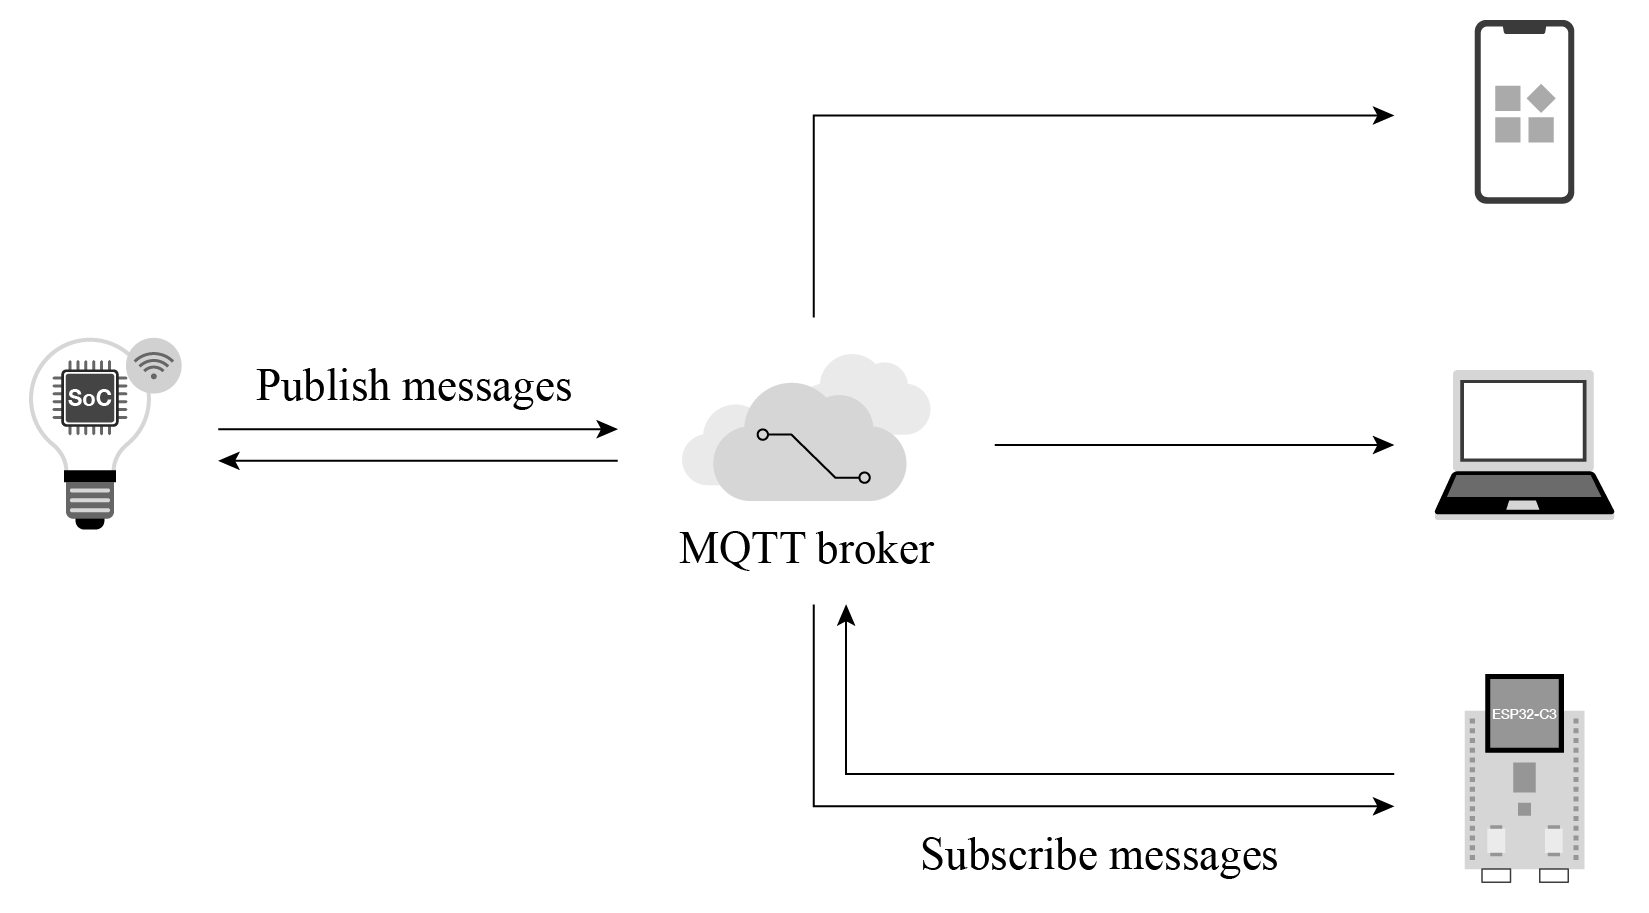
\includegraphics[width=0.72\textwidth]{D9Z/9-1}
    \caption{Architecture of MQTT protocol}
\end{figure}

(1) \textbf{Client}: a device running MQTT applications, such as smartphones and controlled devices. It can work as a publisher or subscriber. A Client always connects to the Server over the network. It can:

\begin{itemize}[noitemsep]
    \item  Publish application messages that other Clients might be interested in.
    \item Subscribe to request application messages that it is interested in receiving.
    \item Unsubscribe to remove a request for application messages.
    \item Disconnect from the Server.
\end{itemize}

(2) \textbf{Server}: a broker that acts as an intermediary between Clients publishing application messages and Clients requesting to subscribe to them, such as cloud platforms and cloud servers. It can:

\begin{itemize}[noitemsep]
    \item Accept network connections from Clients.
    \item Accept application messages published by Clients.
    \item Process subscribe and unsubscribe requests from Clients.
    \item Forward application messages that match Client subscriptions.
\end{itemize}

(3) \textbf{Subscription}: comprising a Topic Filter and a maximum QoS. It is associated with a single Session, while a Session may contain multiple Subscriptions. Each Subscription within a session has a different Topic Filter.

(4) \textbf{Topic}: the label attached to an application message. It is matched against the Subscriptions known to the Server. The Server sends a copy of the application message to each Client that has a matching Subscription.

(5) \textbf{Topic Filter}: an expression contained in a Subscription, indicating an interest in one or more topics. A Topic Filter can include wildcard characters to represent single or multiple characters.

(6) \textbf{Session}: a stateful interaction between a Client and a Server from the start to the end of a connection. Some Sessions last only as long as the Network Connection.

(7) \textbf{Publish/Subscribe}: the core of the MQTT protocol. It allows communication between subscribers and publishers without knowledge of each other’s IP address or port number. Direct connection is not even necessary, and subscribers and publishers can operate without knowing each other's existence. Message exchanges between them are done by the broker, which filters all the published messages and then distributes them to the matching subscribers.

Both subscribers and publishers are concerned about the topic of the message. For example, a smartphone wants to check the status of a smart light A. In this case, the smartphone can act as a subscriber to subscribe to the message with the topic \verb|A/light_state| from the broker. Smart light A can act as a publisher. When its state changes, it publishes a status message with the same topic to the broker. Then, the broker filters subscribers who have subscribed to the topic and publishes the status message to them. In this way, the smartphone can query the status of smart light A.

\subsection{MQTT Message Format}
As defined by the MQTT protocol, an MQTT control packet consists of three parts: fixed header, variable header, and payload.

(1) \textbf{Fixed header}, present in all MQTT control packets.

As shown in Figure 9.2, the packet type takes 4 bits.

\begin{figure}[!h]
    \centering
    
\includegraphics[width=0.8\textwidth]{D9Z/9-2}
    \caption{Fixed header of MQTT control packets}
\end{figure}

There are 14 types of control packets in total, as listed in Table 9.1.

\begin{table}[h!]
    \renewcommand{\arraystretch}{1.2}
    \caption{Types of MQTT control packets}
    \begin{tabular}{|>{\Centering}m{7em}|>{\Centering}m{4em}|>{\Centering}m{9em}|m{18em}|}
        \hline
        \rowcolor{LightBlue} \textbf{Name}&\textbf{Value}&\textbf{Direction of Flow}&\multicolumn{1}{c|}{\textbf{Description}}\\
        \hline
        Reserved&0&Forbidden&Reserved\\
        \hline
        CONNECT&1&Server $\Leftarrow$ Client&Client request to connect to Server\\
        \hline
        CONNACK&2&Server $\Rightarrow$ Client&Connection acknowledgement\\
        \hline
        PUBLISH&3&Server $\Leftrightarrow$ Client&Publish message\\
        \hline
        PUBACK&4&Server $\Leftrightarrow$ Client&Publish of QoS 1 message acknowledged\\
        \hline
        PUBREC&5&Server $\Leftrightarrow$ Client&Publish received (assured delivery part 1)\\
        \hline
        PUBREL&6&Server $\Leftrightarrow$ Client&Publish release (assured delivery part 2)\\
        \hline
        PUBCOMP&7&Server $\Leftrightarrow$ Client&Publish of QoS 2 message complete\newline(assured delivery part 3)\\
        \hline
        SUBSCRIBE&8&Server $\Leftarrow$ Client&Subscribe request of Client\\
        \hline
        SUBACK&9&Server $\Rightarrow$ Client&Subscribe acknowledgement\\
        \hline
        UNSUBSCRIBE&10&Server $\Leftarrow$ Client&Unsubscribe request\\
        \hline
        UNSUBACK&11&Server $\Rightarrow$ Client&Unsubscribe acknowledgement\\
        \hline
        PINGREQ&12&Server $\Leftarrow$ Client&PING request\\
        \hline
        PINGRESP&13&Server $\Rightarrow$ Client&PING response\\
        \hline
        DISCONNECT&14&Server $\Leftarrow$ Client&Client is disconnecting\\
        \hline
    \end{tabular}
\end{table}

There are three MQTT QoS levels: QoS 0, QoS 1, and QoS 2.

\begin{enumerate}[label=\alph*.,leftmargin=1.5em]
    \item \textbf{QoS 0}: delivered once at most.
    
    The transmission of messages is completely dependent on the underlying TCP/IP network. As the MQTT protocol does not define response and retry, the message will either reach the server only once or not at all. The flow of MQTT QoS 0 is shown in Figure 9.3.

    \begin{figure}[!h]
        \centering
        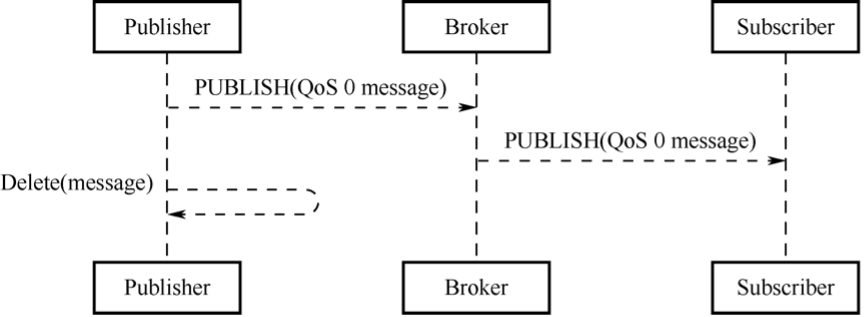
\includegraphics[width=0.7\textwidth]{D9Z/9-3}
        \caption{Flow of MQTT QoS 0}
    \end{figure}

    \item \textbf{QoS 1}: delivered once at least.
    
    The acknowledgement of message receipt is provided by the PUBACK message. If the communication link or the sending device is abnormal, or the message is not received within the specified time, the sender will redeliver the message, and in the fixed header of the MQTT Control packet set the duplicate flag (DUP). The flow of MQTT QoS 1 is shown in Figure 9.4.

    \begin{figure}[!h]
        \centering
        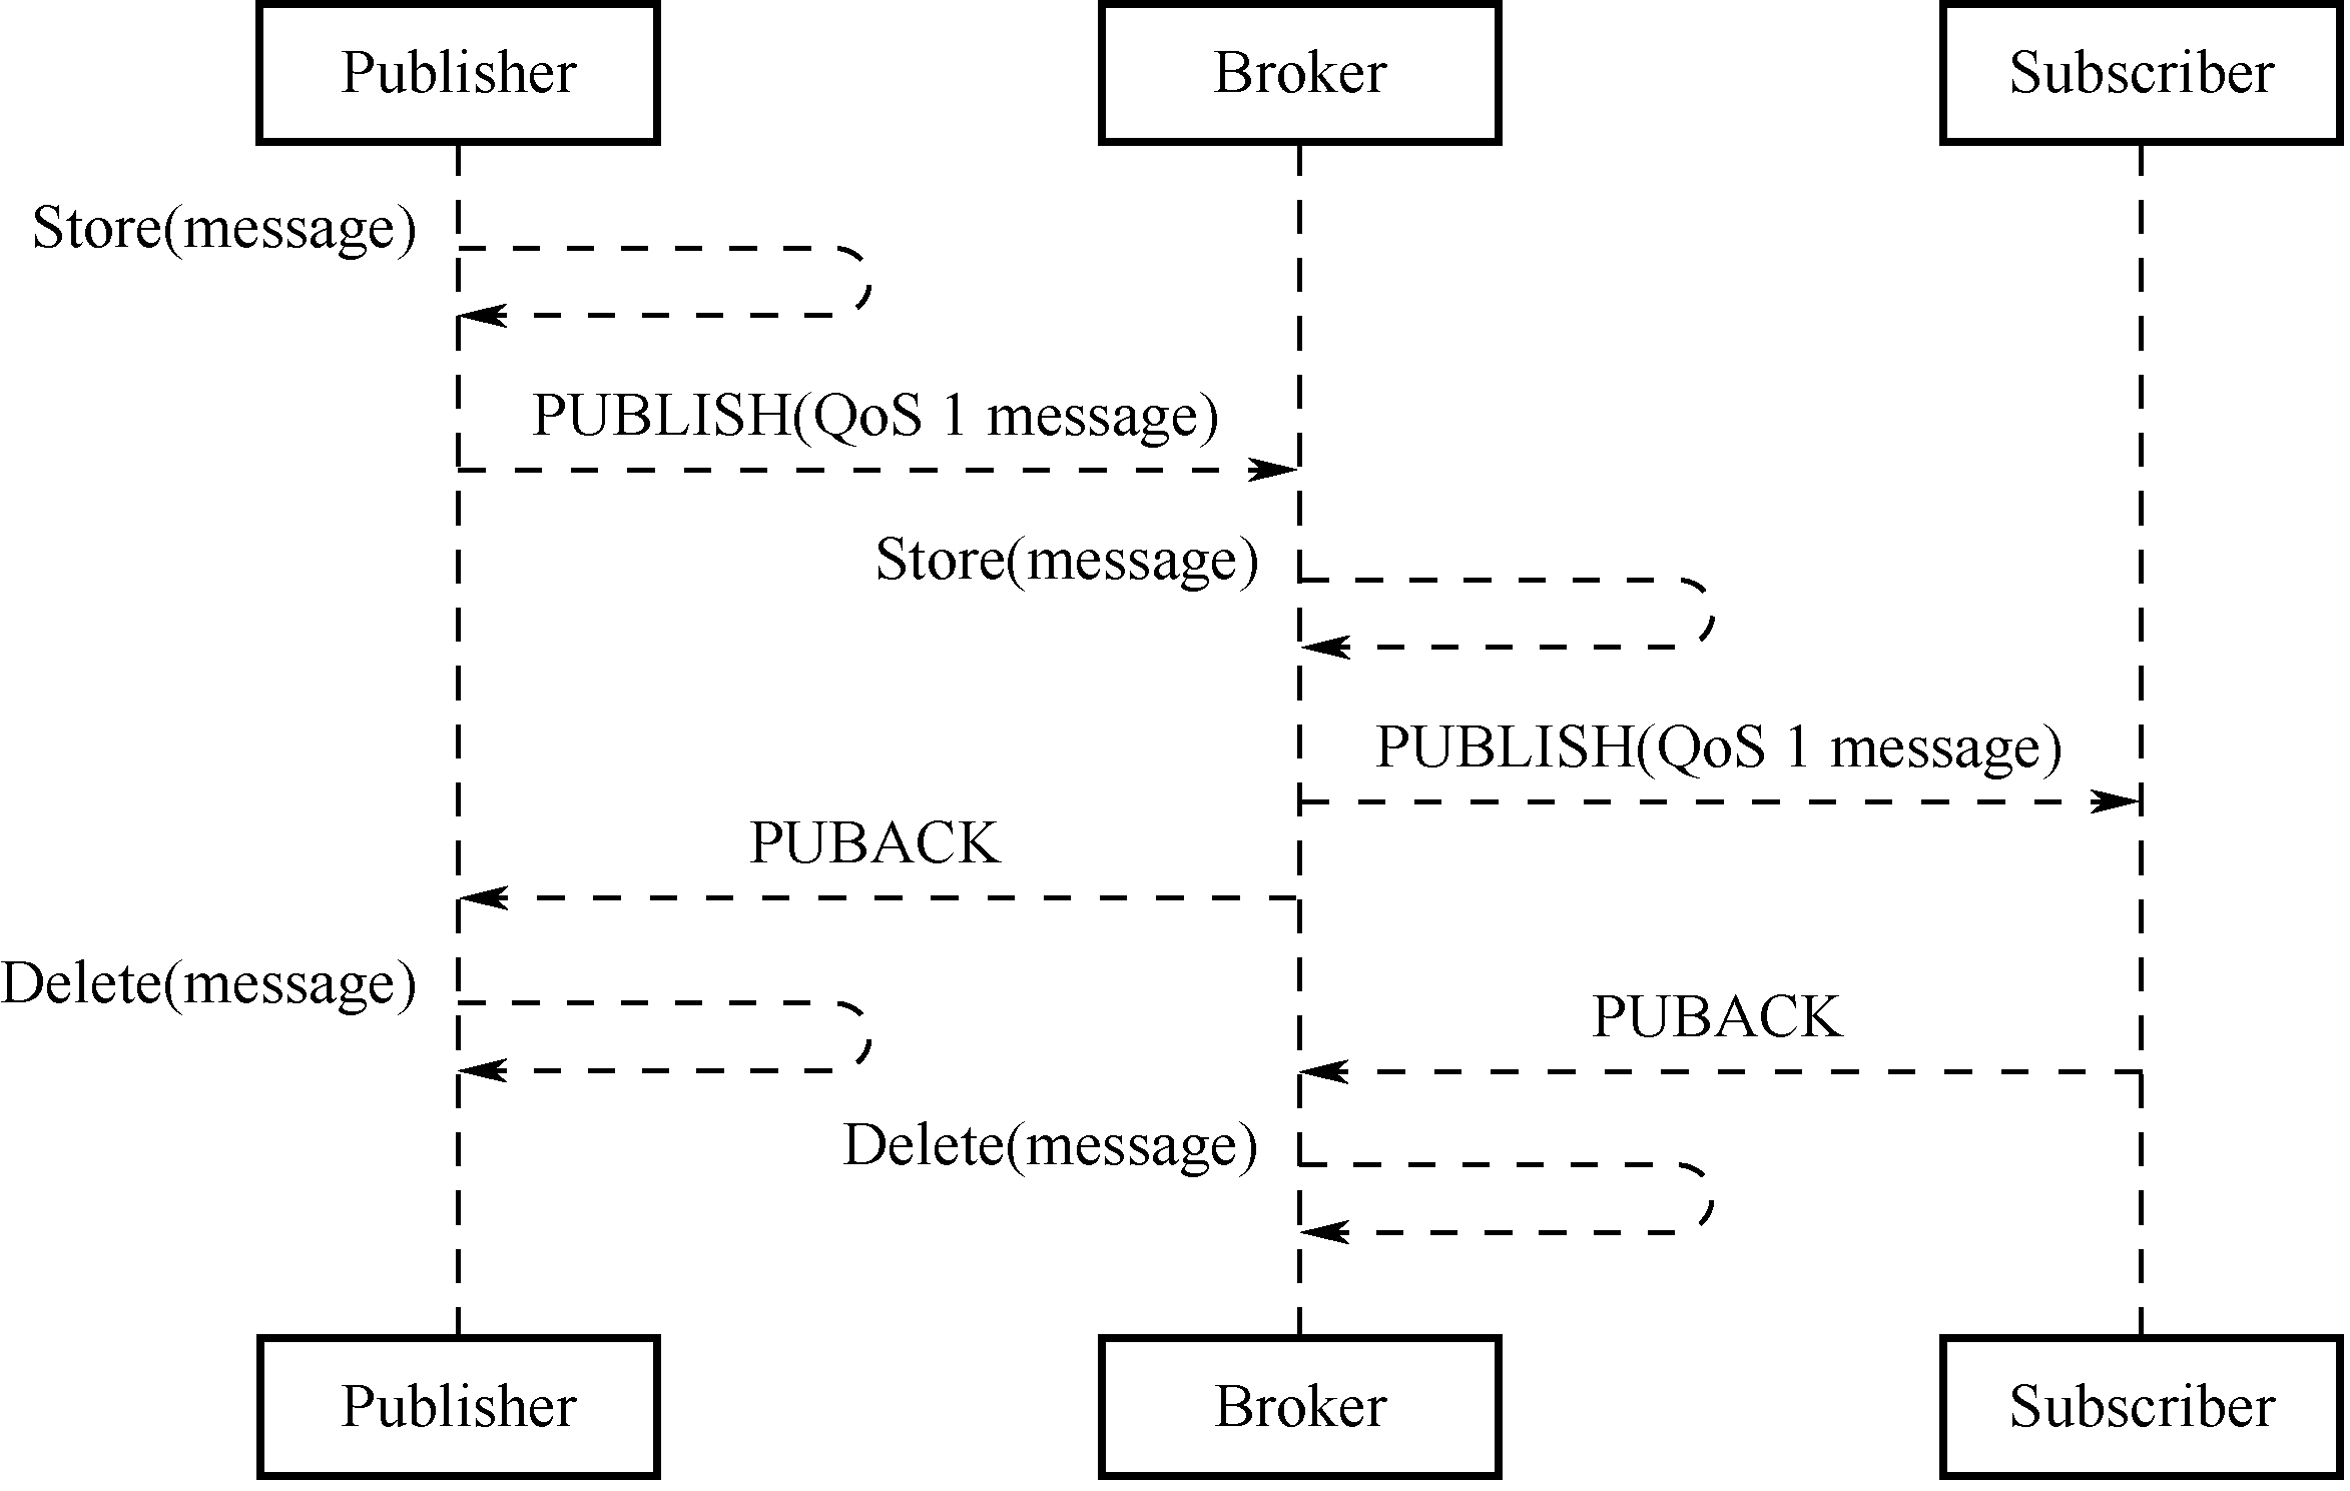
\includegraphics[width=0.7\textwidth]{D9Z/9-4}
        \caption{Flow of MQTT QoS 1}
    \end{figure}

    \item \textbf{QoS 2}: delivered only once.
    
    This is the highest quality of service where message loss and duplication are unacceptable and increased overhead is incurred. The flow of MQTT QoS 2 is shown in Figure 9.5.

    \begin{figure}[!h]
        \centering
        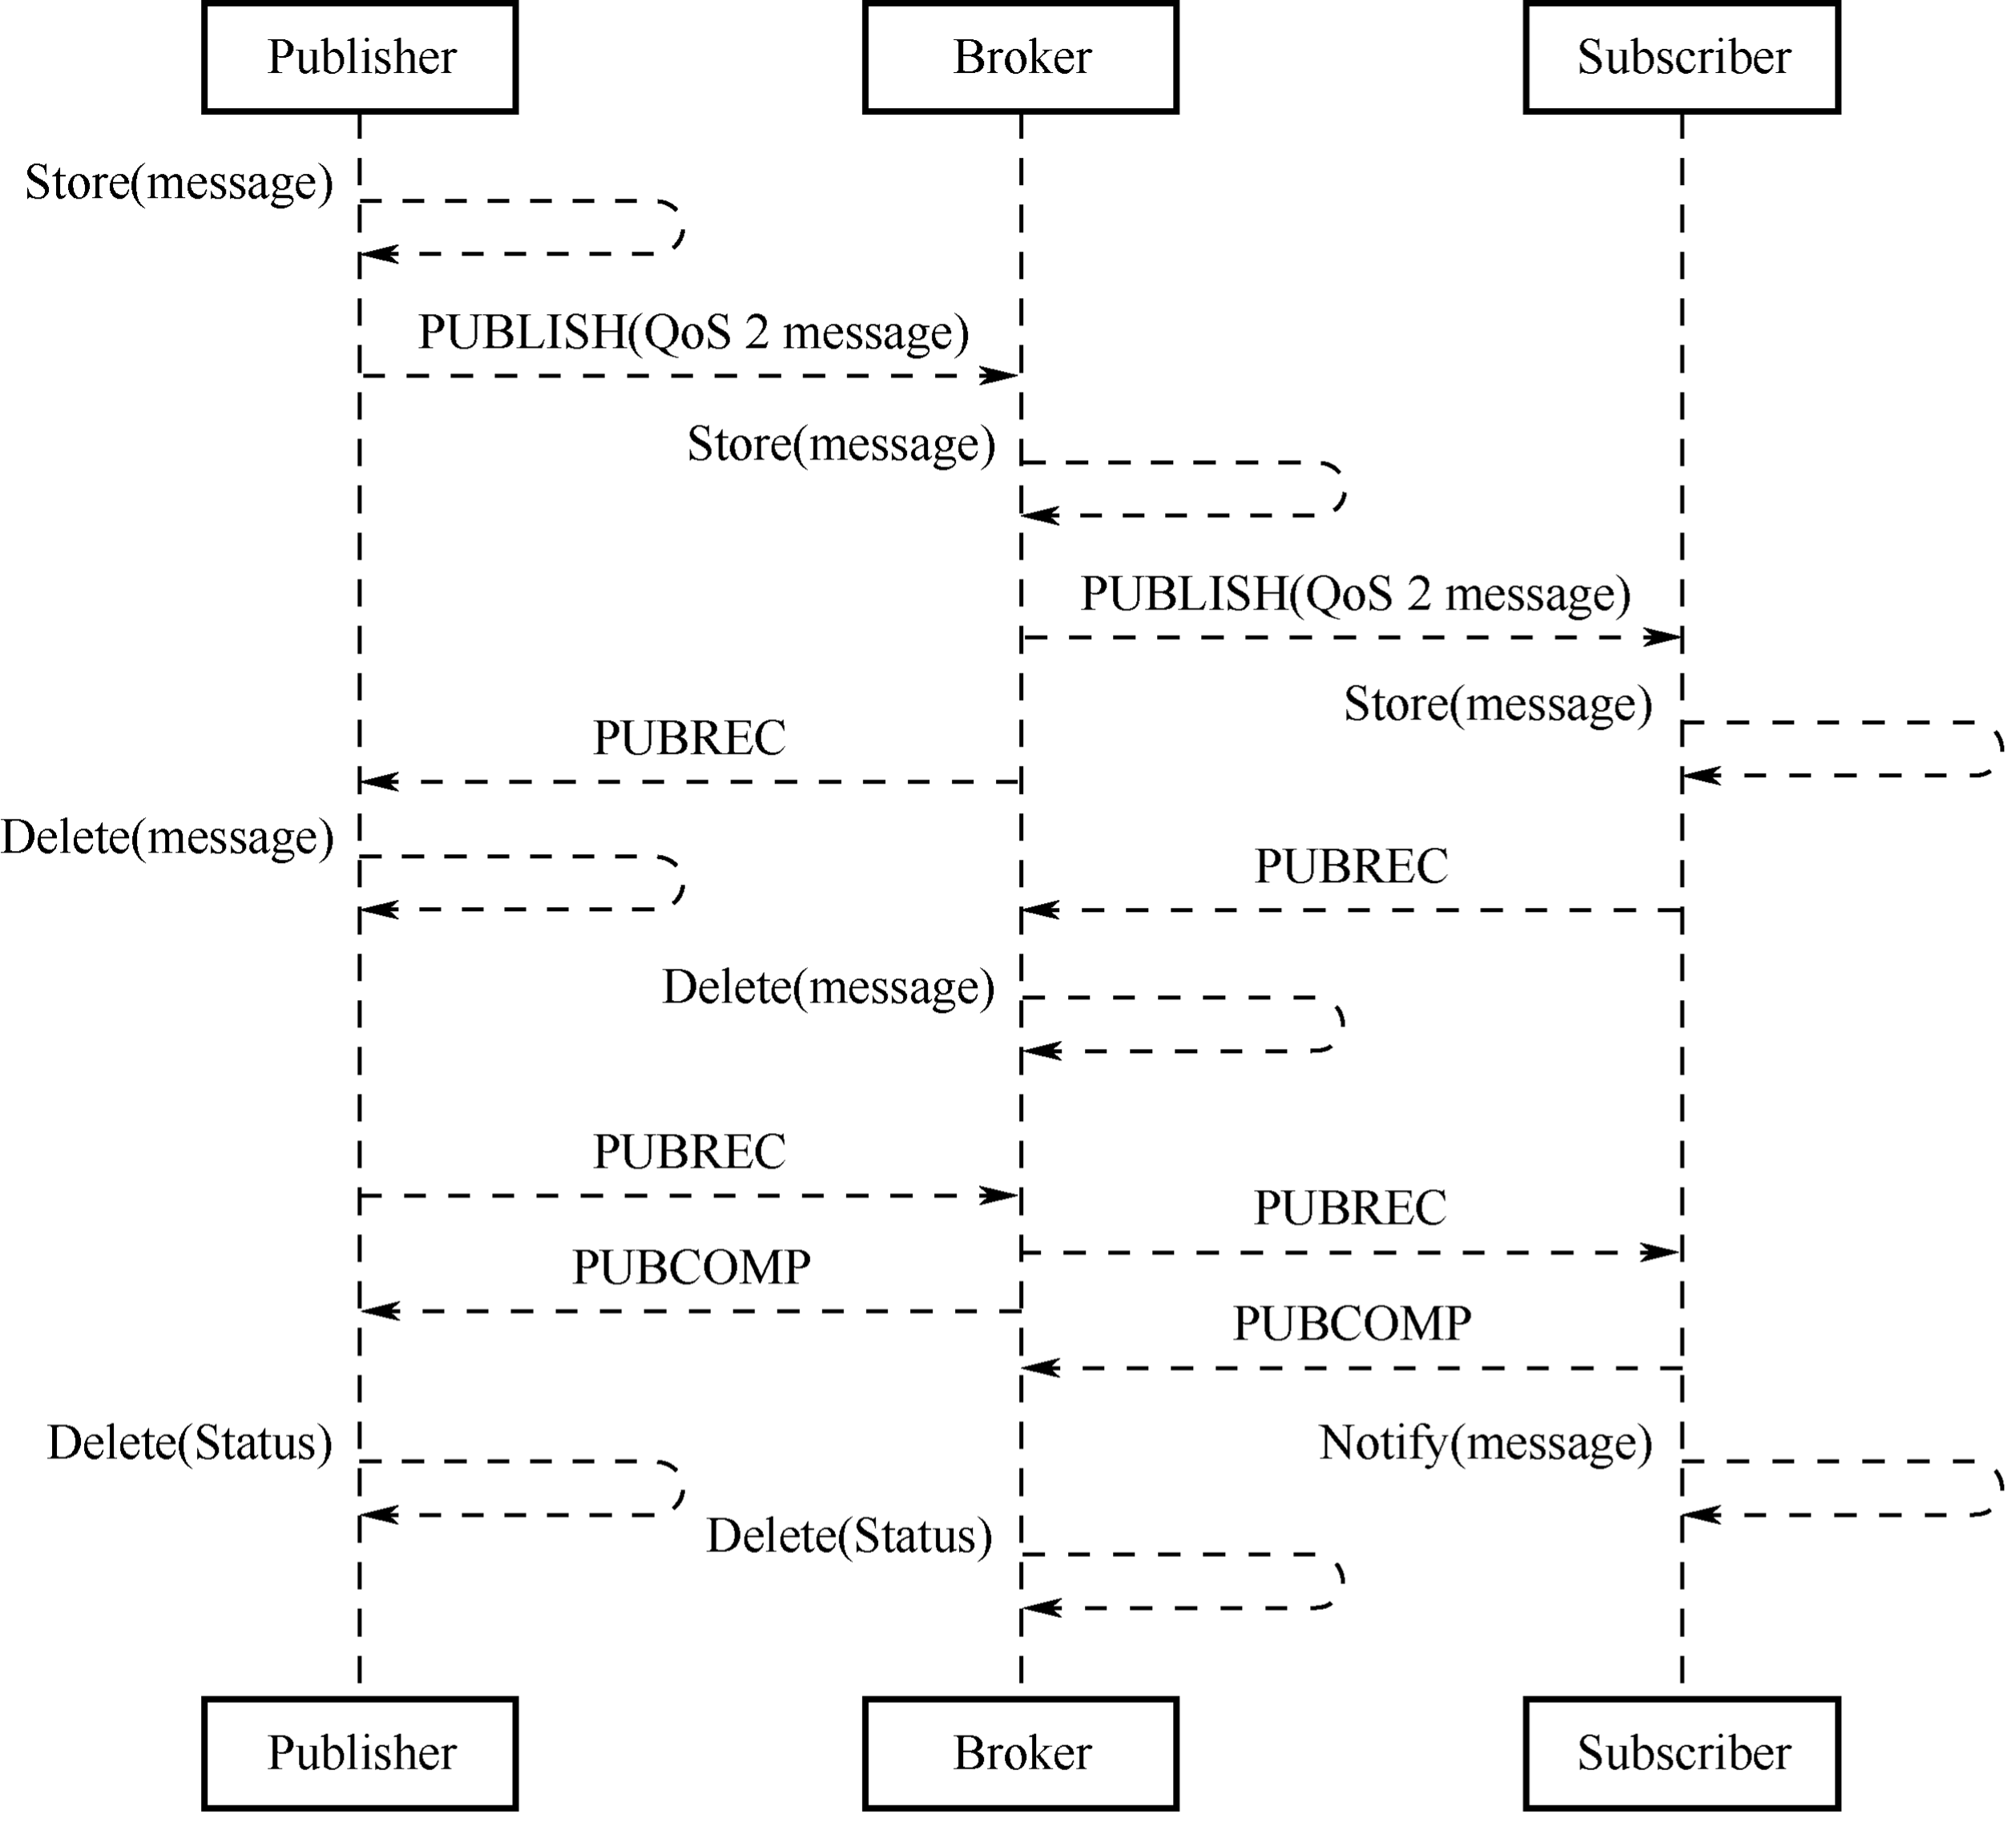
\includegraphics[width=0.7\textwidth]{D9Z/9-5}
        \caption{Flow of MQTT QoS 2}
    \end{figure}
\end{enumerate}

Bits [3–0] of the fixed header contain flags specific to each type of control packets. Except the PUBLISH type, the flag bits of other types are taken by the system. For types without flags, the bits are reserved. If invalid flags are received, the receiver must close the network connection. The bits [3–0] in byte 1 of the PUBLISH packet header are as follows:

\begin{enumerate}[label=\alph*.,leftmargin=1.5em]
    \item \textbf{DUP (bit3)}: duplicate delivery.
    
    “0” means that this is the first time that the Client or Server requests to send a PUBLISH message. “1” indicates that this may be a duplicate delivery of an earlier message. The DUP flag of QoS 0 messages must be set to 0.

    \item \textbf{QoS (bits [2–1])}: determining the number of message delivery.
    
    Table 9.2 shows how to represent QoS values in bits [2–1].

    \begin{table}[h!]
        \renewcommand{\arraystretch}{1.2}
        \caption{Representation of QoS values in bits [2–1]}
        \begin{tabular}{|>{\Centering}m{8em}|>{\Centering}m{8em}|>{\Centering}m{8em}|>{\Centering}m{14em}|}
            \hline
            \rowcolor{LightBlue} \textbf{QoS Value}&\textbf{Bit2}&\textbf{Bit1}&\textbf{Description}\\
            \hline
            0&0&0&Delivered once at most\\
            \hline
            1&0&1&Delivered once at least\\
            \hline
            2&1&0&Delivered only once\\
            \hline
            —&1&1&Reserved\\
            \hline
        \end{tabular}
    \end{table}

    \item \textbf{RETAIN (bit0)}: determining the need for message retaining.
    
    If this flag is set to 1 in a PUBLISH message sent by the Client to the Server, the Server must store this message and its QoS to distribute them later to subscribers with a matching topic. Each Client subscribing to a topic pattern that matches the topic of the retained message receives the retained message immediately after they subscribe. The RETAIN flag is usually used for will messages. For example, after a device is unexpectedly disconnected, the broker will send the will message to the smartphone, where the device will be displayed as offline.
\end{enumerate}

The second and subsequent bytes indicate the remaining length, indicating the number of remaining bytes within the current packet, including data in the variable header and the payload. The remaining length is encoded using a variable-length encoding scheme that uses a single byte for values up to 127. For larger values, the least significant seven bits of each byte encode the data, and the most significant bit is used to indicate whether there are following bytes in the representation. Thus, each byte encodes 128 values and a “continuation bit”. The maximum number of bytes in the remaining length field is 4B. The number of remaining length bytes is shown in Table 9.3.

\begin{table}[h!]
    \renewcommand{\arraystretch}{1.2}
    \caption{Number of remaining length bytes}
    \begin{tabular}{|>{\Centering}m{4em}|m{17em}|m{17em}|}
        \hline
        \rowcolor{LightBlue} \textbf{Byte}&\multicolumn{1}{c|}{\textbf{Minimum Value}}&\multicolumn{1}{c|}{\textbf{Maximum Value}}\\
        \hline
        1&0 (0x00)&127 (0x7F)\\
        \hline
        2&128 (0x80, 0x01)&16383 (0xFF, 0x7F)\\
        \hline
        3&16384 (0x80, 0x80, 0x01)&2097151 (0xFF, 0xFF, 0x7F)\\
        \hline
        4&2097152 (0x80, 0x80, 0x80, 0x01)&268435455 (0xFF, 0xFF, 0xFF, 0x7F)\\
        \hline
    \end{tabular}
\end{table}

(2)	\textbf{Variable header.}

Some types of MQTT Control Packets contain a variable header component. It resides between the fixed header and the payload. The content of the variable header varies depending on the packet type. The Packet Identifier field of the variable header is present in multiple types of packets, such as PUBLISH (when QoS>0), PUBACK, PUBREC, PUBREL, PUBCOMP, SUBSCRIBE, SUBACK, UNSUBSCRIBE, and UNSUBACK.

(3)	\textbf{Payload}: the third part of an MQTT control packet, containing the message content.

It exists in five types of packets, CONNECT, SUBSCRIBE, SUBACK, UNSUBSCRIBE, and PUBLISH.

\begin{enumerate}[label=\alph*.,noitemsep]
    \item CONNECT: Client ID, topic, message, user name, and password.
    \item SUBSCRIBE: a series of topics to subscribe to and the QoS.
    \item SUBACK: the server’s acknowledgment and reply to the topic (that the Client requests to subscribe) and the QoS.
    \item UNSUBSCRIBE: the topics to unsubscribe.
    \item PUBLISH: the to-be-published application message, which can be zero-length.
\end{enumerate}

\subsection{Protocol Comparison}
Chapter 8 introduced protocols such as TCP, HTTP, UDP, and CoAP, which can facilitate local control. In addition, they can also be used for remote control.

\begin{term}{MQTT vs. TCP}
    MQTT is an application protocol based on the TCP protocol. Both can be used for remote data communication. For socket programming, TCP requires users to develop their own application protocols, which have limited usability in the current environment of IoT interconnection. On the other hand, MQTT is a standardized lightweight protocol for IoT and is widely used by most cloud servers, such as Alibaba Cloud and Amazon Cloud, making it advantageous for product integration.
\end{term}

\begin{term}{MQTT vs. HTTP}
    Both are client-server application protocols based on TCP. However, compared to MQTT, HTTP has a much larger overhead in message size, and it is generally difficult for an HTTP server to initiate data push to clients, which may not meet the requirements of remote control in IoT. In cases where only one-way transmission from clients to the server is needed, HTTP protocol can be used.
\end{term}

\begin{term}{MQTT vs. CoAP}
    Similar to HTTP, CoAP adopts the REST model where the server creates resources in URI format and clients access these resources using GET, PUT, POST, and DELETE methods. Besides, CoAP also has a similar protocol style to HTTP, but it requires fewer device resources and network overheads, making it suitable for IoT. However, CoAP may not be a good choice for remote control. If smartphones send control commands for remote control, the architecture may require CoAP + Web + Database + App. When CoAP protocol is used, control commands must pass through the Database before reaching the device, because CoAP is connectionless. When smartphones send control commands, the server will first store the control commands in the Database, and the device will request the server via GET method to check if there are any control commands, and then decide whether to operate. On the other hand, MQTT is connection-oriented, and the server will forward the control commands from smartphones to all subscribed devices without storing them. Only MQTT client + MQTT server + App is needed to implement remote control, making MQTT more advantageous in terms of deployment.
\end{term}

\subsection{Setting Up MQTT Broker on Linux and Windows}
Some commonly used MQTT brokers are Mosquitto, EMQTT, and HiveMQ. HiveMQ is not open-source and has a fee, so it may not be suitable for local testing. EMQTT has powerful features, such as viewing data traffic on a web interface, and can be used on most cloud servers, with both free and paid custom versions available.

This section focuses on how to use Mosquitto to set up an MQTT broker on Windows or Linux. Mosquitto is an open-source (EPL/EDL licensed) message broker that implements MQTT protocol versions 5.0, 3.1.1, and 3.1. It is considered a lightweight open-source software. The Mosquitto project provides a C language library for implementing MQTT clients and popular command-line MQTT clients \verb|mosquitto_pub| and \verb|mosquitto_sub|. Besides, Mosquitto can also be used as an MQTT broker. For more information, please refer to its official website.

\textbf{1. Setting up MQTT broker on Linux}

All terminal commands in this section must be run in the user role. The \verb|$| symbol represents the command prompt.

(1) Download \textbf{mosquitto-2.0.12.tar.gz} from \url{https://mosquitto.org/files/source}.

(2)	Extract Mosquitto.

\begin{codebloc}
\begin{tabular}{d}
\$ \textbf{tar -zxvf mosquitto-2.0.12.tar.gz}
\end{tabular}
\end{codebloc}

Check if the installation is successful using \verb|mosquitto --help|.

\begin{codebloc}
\begin{tabular}{d}
\$ \textbf{cd mosquitto-2.0.12/src}

\$ \textbf{mosquitto --help}
\begin{verbatim}
mosquitto version 2.0.12
mosquitto is an MQTT v5.0/v3.1.1/v3.1 broker. 
    Usage: mosquitto [-c config_file] [-d] [-h] [-p port]
        -c : specify the broker config file.
        -d : put the broker into the background after starting.
        -h : display this help.
        -p : start the broker listening on the specified port.
          Not recommended in conjunction with the -c option.
        -v : verbose mode - enable all logging types. This overrides
          any logging options given in the config file.
\end{verbatim}
\verb|        See https://mosquitto.org/ for more information.|
\end{tabular}
\end{codebloc}

(3) Start MQTT broker and test in the MQTT client.

a. Start MQTT.

\begin{codebloc}
\begin{tabular}{d}
\$ \textbf{mosquitto}
\end{tabular}
\end{codebloc}

b. Use \verb|mosquitto_sub| to subscribe to \verb|topic|.

\begin{codebloc}
\begin{tabular}{d}
\$ \textbf{mosquitto\_sub -t ‘test/topic’ -v}
\end{tabular}
\end{codebloc}

c. Open a new terminal and use \verb|mosquitto_pub| to publish data.

\begin{codebloc}
\begin{tabular}{d}
\$ \textbf{mosquitto\_pub -t ‘test/topic’ -m ‘hello world’}
\end{tabular}
\end{codebloc}

d. In the original terminal where the \verb|topic| was subscribed, view the received data.

\begin{codebloc}
\begin{tabular}{d}
\$ \textbf{mosquitto\_sub -t ‘test/topic’ -v}

test/topic hello world
\end{tabular}
\end{codebloc}

\textbf{2. Setting up MQTT broker on Windows}

(1) Download the 32-bit or 64-bit MQTT installation package based on your computer’s architecture. Double-click to install it.

(2) Open a command prompt window, navigate to the directory where Mosquitto is installed, and start the Mosquitto broker.

\begin{codebloc}
\begin{tabular}{d}
\textbf{cd C:$\setminus$Program Files$\setminus$mosquitto$\setminus$}
\end{tabular}
\end{codebloc}

(3) Use \verb|mosquitto_sub.exe| to subscribe to \verb|topic|.

\begin{codebloc}
\begin{tabular}{d}
\textbf{C:$\setminus$Program Files$\setminus$mosquitto>mosquitto\_sub.exe -t ‘test/topic’ -v}
\end{tabular}
\end{codebloc}

(4) Use \verb|mosquitto_pub.exe| to publish data.

\begin{codebloc}
\begin{tabular}{d}
\textbf{C:$\setminus$Program Files$\setminus$mosquitto>mosquitto\_pub.exe -t ‘test/topic’ -m ‘hello\_world’}
\end{tabular}
\end{codebloc}

\subsection{Setting Up MQTT Client Based on ESP-IDF}
The component used in ESP-IDF to implement MQTT client is ESP-MQTT, which has the following features:

\begin{itemize}[noitemsep]
    \item Support for MQTT, MQTT over TLS, MQTT over WebSocket, and MQTT over WebSocket, and TLS
    \item Easy to set up with URI
    \item Multiple clients in one application
    \item Support for subscribing, publishing, authentication, last will messages, keep-alive pings, and QoS messages
\end{itemize}

The following code is based on ESP-IDF and creates a connection to a local MQTT broker. For complete code, please go to ESP-IDF project on GitHub and navigate to the directory \href{https://github.com/espressif/esp-idf/tree/master/examples/protocols/mqtt/tcp}{\texttt{esp-idf/examples/protocols/mqtt/tcp}}.

\begin{codebloc}
\begin{tabular}{d}
\vspace{2pt}
\begin{verbatim}
1.  //MQTT event handler function
2.  static void mqtt_event_handler(void *handler_args, esp_event_base_t base,
3.                                 int32_t event_id, void *event_data)
4.  {
5.      esp_mqtt_event_handle_t event = event_data;
6.      esp_mqtt_client_handle_t client = event->client;
7.      int msg_id;
8.      switch ((esp_mqtt_event_id_t)event_id) {
9.          case MQTT_EVENT_CONNECTED:
10.         ESP_LOGI(TAG, "MQTT_EVENT_CONNECTED");
11.         //Subscribe to topic /topic/test
12.         msg_id = esp_mqtt_client_subscribe(client, "/topic/test", 0);
13.         ESP_LOGI(TAG, "sent subscribe successful, msg_id=%d", msg_id);
14.         break;
15.         case MQTT_EVENT_DISCONNECTED:
\end{verbatim}
\verb|16.         ESP_LOGI(TAG, "MQTT_EVENT_DISCONNECTED");|
\end{tabular}
\end{codebloc}

\begin{codebloc}
\begin{tabular}{d}
\vspace{2pt}
\begin{verbatim}
17.         break;
18.         case MQTT_EVENT_SUBSCRIBED:
19.         ESP_LOGI(TAG, "MQTT_EVENT_SUBSCRIBED, msg_id=%d", event->msg_id);
20.         break;
21.         case MQTT_EVENT_UNSUBSCRIBED:
22.         ESP_LOGI(TAG, "MQTT_EVENT_UNSUBSCRIBED, msg_id=%d", event->msg_id);
23.         break;
24.         case MQTT_EVENT_PUBLISHED:
25.         ESP_LOGI(TAG, "MQTT_EVENT_PUBLISHED, msg_id=%d", event->msg_id);
26.         break;
27.         case MQTT_EVENT_DATA:
28.         ESP_LOGI(TAG, "MQTT_EVENT_DATA");
29.         ESP_LOGI(TAG, "TOPIC=%.*s\r\n", event->topic_len, event->topic);
30.         ESP_LOGI(TAG, "DATA=%.*s\r\n", event->data_len, event->data);
31.         break;
32.         case MQTT_EVENT_ERROR:
33.         ESP_LOGI(TAG, "MQTT_EVENT_ERROR");
34.         break;
35.         default:
36.         ESP_LOGI(TAG, "Other event id:%d", event->event_id);
37.         break;
38.     }
39. }
40.
41. #define CONFIG_BROKER_URL "mqtt://192.168.3.4/"
42.
43. static void esp_mqtt_start(void)
44. {
45.     //Configure MQTT URI
46.     esp_mqtt_client_config_t mqtt_cfg = {
47.         .uri = CONFIG_BROKER_URL,
48.     };
49.
50.     //Initialise MQTT client
51.     esp_mqtt_client_handle_t client = esp_mqtt_client_init(&mqtt_cfg);
52.
53.     //Register event handler function
\end{verbatim}
\verb|54.     |\fontsize{8.5pt}{8.5pt}\selectfont\verb|esp_mqtt_client_register_event(client, ESP_EVENT_ANY_ID, mqtt_event_handler, NULL);|
\footnotesize
\begin{verbatim}
55.
56.     //Start MQTT client
57.     esp_mqtt_client_start(client);
\end{verbatim}
\verb|58. }|
\end{tabular}
\end{codebloc}

The client device connects to the MQTT broker and subscribes to the topic \verb|/topic/test|. After another MQTT client publishes the message \verb|hello world| to the topic \verb|/topic/test|, the following log will show up in the device:

\begin{codebloc}
\begin{tabular}{d}
\verb|I (2598) wifi station: MQTT_EVENT_CONNECTED|
\end{tabular}
\end{codebloc}

\begin{codebloc}
\begin{tabular}{d}
\vspace{2pt}
\begin{verbatim}
I (2598) wifi station: sent subscribe successful, msg_id=25677
I (2648) wifi station: MQTT_EVENT_SUBSCRIBED, msg_id=25677
I (314258) wifi station: MQTT_EVENT_DATA
I (314258) wifi station: TOPIC=/topic/test
\end{verbatim}
\verb|I (314258) wifi station: DATA=hello world|
\end{tabular}
\end{codebloc}

\section{Ensuring MQTT Data Security}
Data transmitted using the MQTT protocol is in plain text, which means it can be intercepted if not encrypted. In Chapter 8.4.1, the TLS protocol is introduced as a means to ensure that data can only be decrypted by the communicating parties, thereby safeguarding data security and legitimacy.

Similarly, TLS can also be used for encryption in cloud communication over MQTT. Since it has already been covered in Chapter 8.4.1, this section only introduces what the certificates in the TLS handshake mean and what functions they perform, how to generate certificates locally, and how to set up a mutual authentication TLS environment based on the local MQTT broker.

\subsection{Meaning and Function of Certificates}
\textbf{1.	Introduction}

Certificates, also known as public-key certificates (PKC), contain personal information such as user name, organization, email, the user’s public key, and the digital signature of a certification authority or certifying authority (CA). You can think of a certificate as a personal identity card, with the public key serving as the card number, identifying which individual it represents. A CA is like a police station that issues the card. It can be an international organization, government entity, for-profit company, or general individual.

\textbf{2.	Certificate generation}

\begin{enumerate}[label=(\arabic*)]
    \item User A generates a private-public key pair locally using an asymmetric encryption algorithm.
    \item User A submits the locally generated public key and certificate information file to a CA for digital signing and certificate generation. 
    \item The CA generates a private-public key pair locally, which is the \verb|ca.key| mentioned in a later example. The CA uses its private key to digitally sign User A’s public key and issues the certificate.
    \item User B obtains the CA’s public key, which is publicly available, and uses it to verify the legitimacy of the digital signature in User A’s certificate. If the verification is successful, it is confirmed that the public key in User A’s certificate belongs to User A.
    \item To send data to User A, User B only needs to encrypt the data using the public key in User A’s certificate and send it. User A then decrypts the data with its own private key.
\end{enumerate}

So far, we have covered the generation of User A’s certificate and the data communication process between User A and User B. However, it only involves one-way authentication of TLS certificate—User A is like the server side, User B is like the client side, and this process can be considered as the client’s verification of the server’s certificate. A similar process is followed for the server’s verification of the client’s certificate.

\textbf{3.	Certificate function}

As indicated by the above certificate generation process, certificates are a means to verify the legitimacy of the peer device. Only when it is legitimate can the transmitted data can be secured without the risk of being leaked.

\textbf{4.	Certificate standard}

Certificates adopt the common format X.509. All certificates comply with the ITU-T X.509 international standard. The structure of X.509 certificates is described and encoded using Abstract Syntax Notation One (ASN1). 

A certificate typically consists of the following fields:

\begin{itemize}[leftmargin=1.5em,noitemsep]
    \item \textbf{Version Number}: the version number of the specification. The current version is 3, corresponding to the value 0x2.
    \item \textbf{Serial Number}: the unique serial number maintained by the CA and assigned to each certificate for tracking and revocation. The maximum size is 20 bytes.
    \item \textbf{Signature Algorithm}: the algorithm used for digital signatures.
    \item \textbf{Validity}: the validity period of the certificate, including start and end dates.
    \item \textbf{Subject}: the identifier information of the certificate holder, namely the personal information mentioned above.
    \item \textbf{Subject Public Key Info}: protected information related to the public key, including the public key algorithm and subject unique identifier.
\end{itemize}

\textbf{5.	Certificate format}

Privacy Enhanced Mail (PEM) is a common format for X.509 certificates. PEM files are usually seen with the extensions \verb|.crt| or \verb|.cer| (for certificates), \verb|.key| (for private keys), and \verb|.csr| (for certificate signing request).

The PEM file is a text file that usually contains headers, footers, and the content blocks encoded in Base64.

\subsection{Generating Certificates Locally}
OpenSSL is an open-source Secure Socket Layer (SSL) cryptographic library that provides functions for algorithms, key and certificate encapsulation management, and SSL protocol implementation. It consists of three parts: an SSL protocol library, command-line tools for applications, and cryptographic algorithm libraries. The following examples demonstrate how use it to generate certificates and keys on Linux.

\textbf{1.	Generating private keys for the certificate}

This command generates a private key (2048 bits) for the certificate. The public key can be extracted from it.

\begin{codebloc}
\begin{tabular}{d}
\$ \textbf{openssl genrsa -out ca.key 2048}
\begin{verbatim}
Generating RSA private key, 2048 bit long modulus
...............................................................................
............................................+++
.......+++
\end{verbatim}
\verb|e is 65537 (0x10001)|
\end{tabular}
\end{codebloc}

This command generates a private key (2048 bits) for the server certificate.

\begin{codebloc}
\begin{tabular}{d}
\$ \textbf{openssl genrsa -out server.key 2048}
\begin{verbatim}
Generating RSA private key, 2048 bit long modulus
................+++
........................+++
\end{verbatim}
\verb|e is 65537 (0x10001)|
\end{tabular}
\end{codebloc}

This command generates a private key (2048 bits) for the client certificate.

\begin{codebloc}
\begin{tabular}{d}
\$ \textbf{openssl genrsa -out client.key 2048}
\begin{verbatim}
Generating RSA private key, 2048 bit long modulus
...............................................+++
........................................................+++
\end{verbatim}
\verb|e is 65537 (0x10001)|
\end{tabular}
\end{codebloc}

The recommended minimum key length for RSA algorithm is 2048 bits. If the key length is 1024 bits, \verb|mbedtls| will reject TLS negotiation due to low security.

\textbf{2. Generating CSRs for the certificate}

This command generates a certificate sign request (CSR) that is required by the CA certificate. Enter the required information as prompted. The \verb|Organization Name| can be entered as desired because this is only for local use.

\begin{codebloc}
\begin{tabular}{d}
\$ \textbf{openssl req -out ca.csr -key ca.key -new}
\begin{verbatim}
You are about to be asked to enter information that will be incorporated into
your certificate request.
What you are about to enter is what is called a Distinguished Name or a DN.
There are quite a few fields but you can leave some blank
\end{verbatim}
\verb|For some fields there will be a default value,|
\end{tabular}
\end{codebloc}

\begin{codebloc}
\begin{tabular}{d}
If you enter ‘.’, the field will be left blank.\newline
-----\newline
Country Name (2 letter code) [AU]:\textbf{CN}\newline
State or Province Name (full name) [Some-State]:\newline
Locality Name (eg, city) []:\newline
Organization Name (eg, company) [Internet Widgits Pty Ltd]:\textbf{IOT Certificate Test}\newline
Organizational Unit Name (eg, section) []:\newline
Common Name (e.g. server FQDN or YOUR name) []:\newline
Email Address []:\newline
\vspace{10pt}
Please enter the following ‘extra’ attributes\newline
to be sent with your certificate request\newline
A challenge password []:\newline
An optional company name []:
\end{tabular}
\end{codebloc}

\vspace{6pt}
This command generates a CSR that is required by the server certificate. Note that the \verb|Common Name| field should be filled with the domain name or IP address of the server.

\begin{codebloc}
\begin{tabular}{d}
\$ \textbf{openssl req -out server.csr -key server.key -new}
\begin{verbatim}
You are about to be asked to enter information that will be incorporated into
your certificate request.
What you are about to enter is what is called a Distinguished Name or a DN.
There are quite a few fields but you can leave some blank
For some fields there will be a default value,
If you enter ‘.’, the field will be left blank.
-----
\end{verbatim}
Country Name (2 letter code) [AU]:\textbf{CN}\newline
State or Province Name (full name) [Some-State]:\newline
Locality Name (eg, city) []:\newline
Organization Name (eg, company) [Internet Widgits Pty Ltd]:\textbf{MQTT Server}\newline
Organizational Unit Name (eg, section) []:\newline
Common Name (e.g. server FQDN or YOUR name) []:\textbf{192.168.3.4}\newline
Email Address []:\newline
\vspace{10pt}
Please enter the following ‘extra’ attributes\newline
to be sent with your certificate request\newline
A challenge password []:\newline
An optional company name []:
\end{tabular}
\end{codebloc}

\vspace{6pt}
\textbf{3.	Generating CA certificate, server certificate, and client certificate}

This command generates the CA certificate \verb|ca.crt|.

\begin{codebloc}
\begin{tabular}{d}
\$ \textbf{openssl x509 -req -in ca.csr -out ca.crt -sha256 -days 5000 -signkey ca.key}\newline
Signature ok\newline
subject=/C=CN/ST=Some-State/O=IOT Certificate Test\newline
Getting Private key
\end{tabular}
\end{codebloc}

\vspace{6pt}
This command generates the server certificate \verb|server.crt|.

\begin{codebloc}
\begin{tabular}{d}
\$ \textbf{openssl x509 -req -in server.csr -out server.crt -sha256 -CAcreateserial -days 5000 -CA ca.crt -CAkey ca.key}\newline
Signature ok\newline
subject=/C=CN/ST=Some-State/O=MQTT Server/CN=192.168.3.4\newline
Getting CA Private Key
\end{tabular}
\end{codebloc}

\vspace{6pt}
This command generates the client certificate \verb|client.crt|.

\begin{codebloc}
\begin{tabular}{d}
\$ \textbf{openssl x509 -req -in client.csr -out client.crt -sha256 -CAcreateserial -days 5000 -CA ca.crt -CAkey ca.key}\newline
Signature ok\newline
subject=/C=CN/ST=Some-State/O=MQTT Client/CN=192.168.3.5\newline
Getting CA Private Key
\end{tabular}
\end{codebloc}

\note{\fontsize{11.5pt}{11.5pt}\selectfont Do not use the SHA1 algorithm, as \texttt{mbedtls} may reject TLS negotiation due to low security.}

\subsection{Configuring MQTT Broker}
Section 9.2.5 described how to set up an MQTT broker on Windows or Linux using Mosquitto, and this section will introduce how to do it over TLS.

Firstly, in the root directory of \verb|mosquitto|, open the configuration file \verb|mosquitto.conf|, and add the absolute path to the files that are generated in Section 9.3.2, including the CA certificate (\verb|ca.crt|), the server certificate (\verb|server.crt|), and the private key of the server certificate (\verb|server.key|). The command is as follows:

\begin{codebloc}
\begin{tabular}{d}
\$ \textbf{port 8883}
\begin{verbatim}
certfile {absolute path}/server.crt
keyfile {absolute path}/server.key
cafile {absolute path}/ca.crt
require_certificate true
\end{verbatim}
\verb|use_identity_as_username true|
\end{tabular}
\end{codebloc}

Then, restart Mosquitto and load the configuration file.

\begin{codebloc}
\begin{tabular}{d}
\$ \textbf{mosquitto -c mosquitto.conf -v}
\begin{verbatim}
1635927859: mosquitto version 1.6.3 starting
1635927859: Config loaded from mosquitto.conf.
1635927859: Opening ipv4 listen socket on port 8883.
\end{verbatim}
\verb|1635927859: Opening ipv6 listen socket on port 8883.|
\end{tabular}
\end{codebloc}

\subsection{Configuring MQTT Client}
In Section 9.2.5, we have covered how to set up an MQTT client based on ESP-IDF using MQTT over TCP, but this approach cannot guarantee data security. So, in this section, we will introduce a more secure approach, which is setting up the client using MQTT over TLS. 

\begin{codebloc}
\begin{tabular}{d}
\vspace{2pt}
\begin{verbatim}
1.extern const uint8_t client_cert_pem_start[] asm("_binary_client_crt_start");
2.  extern const uint8_t client_cert_pem_end[] asm("_binary_client_crt_end");
3.  extern const uint8_t client_key_pem_start[] asm("_binary_client_key_start");
4.  extern const uint8_t client_key_pem_end[] asm("_binary_client_key_end");
5.  extern const uint8_t server_cert_pem_start[] asm("_binary_ca_crt_start");
6.  extern const uint8_t server_cert_pem_end[] asm("_binary_ca_crt_end");
7.
8.  #define CONFIG_BROKER_URL "mqtts://192.168.3.4/"
9.
10. //Configure MQTT URI
11. esp_mqtt_client_config_t mqtt_cfg = {
12.     .uri = CONFIG_BROKER_URL,
13.     .client_cert_pem = (const char *)client_cert_pem_start,
14.     .client_key_pem = (const char *)client_key_pem_start,
15.     .cert_pem = (const char *)server_cert_pem_start,
\end{verbatim}
\verb|16. };|
\end{tabular}
\end{codebloc}

\vspace{6pt}
\begin{enumerate}[label=(\arabic*),noitemsep]
    \item Load the client certificate (\verb|client.crt|), the client private key (\verb|client.key|), and the CA certificate that authenticates the server (\verb|ca.crt|).
    \item Change the previous MQTT connection to \verb|mqtts|.
    \item Use the default port number \verb|8883|. 
    \item Modify the \verb|CMakeLists.txt| file to load the certificates into the firmware during compilation. The code is as follows:
\end{enumerate}

\begin{codebloc}
\begin{tabular}{d}
\verb|1.  target_add_binary_data(${CMAKE_PROJECT_NAME}.elf "main/client.crt" TEXT)|\newline
\verb|2.  target_add_binary_data(${CMAKE_PROJECT_NAME}.elf "main/client.key" TEXT)|\newline
\verb|3.  target_add_binary_data(${CMAKE_PROJECT_NAME}.elf "main/ca.crt" TEXT)|
\end{tabular}
\end{codebloc}

After compilation and flashing, connect the device to Wi-Fi. Then, both the client and server will show a successful connection log, and the client will subscribe to the topic \verb|/topic/test|. The server’s log is as follows:

\begin{codebloc}
\begin{tabular}{d}
\vspace{2pt}
\begin{verbatim}
1635927859: mosquitto version 1.6.3 starting
1635927859: Config loaded from mosquitto.conf.
1635927859: Opening ipv4 listen socket on port 8883.
1635927859: Opening ipv6 listen socket on port 8883.
1635927867: New connection from 192.168.3.5 on port 8883.
1635927869: New client connected from 192.168.3.5 as ESP32_2465F1 (p2, c1, k120, 
u'192.168.3.5').
1635927869: No will message specified.
1635927869: Sending CONNACK to ESP32_2465F1 (0, 0)
1635927869: Received SUBSCRIBE from ESP32_2465F1
1635927869:     /topic/test (QoS 0)
1635927869: ESP32_2465F1 0 /topic/test
\end{verbatim}
\verb|1635927869: Sending SUBACK to ESP32_2465F1|
\end{tabular}
\end{codebloc}

Now, use \verb|mosquitto_pub| to send “hello world” to the topic \verb|/topic/test|. Check if the device can receive it. The command is as follows:

\begin{codebloc}
\begin{tabular}{d}
\$ \textbf{mosquitto\_pub -h 192.168.3.4 -p 8883 -t “/topic/test” -m ‘hello world’ --cafile ca.crt --cert client.crt --key client.key}
\end{tabular}
\end{codebloc}

Here is the log on the device side:

\begin{codebloc}
\begin{tabular}{d}
\vspace{2pt}
\fontsize{9pt}{9.5pt}\selectfont
\begin{verbatim}
I (1600) esp_netif_handlers: sta ip: 192.168.3.5, mask: 255.255.255.0, gw: 192.168.3.1
I (1600) wifi station: got ip:192.168.3.5
I (1600) wifi station: connected to ap SSID:myssid password:12345678
I (1610) wifi station: Other event id:7
W (1630) wifi:<ba-add>idx:0 (ifx:0, 34:29:12:43:c5:40), tid:0, ssn:4, winSize:64
I (4110) wifi station: MQTT_EVENT_CONNECTED
I (4120) wifi station: sent subscribe successful, msg_id=42634
I (4140) wifi station: MQTT_EVENT_SUBSCRIBED, msg_id=42634
I (10290) wifi station: MQTT_EVENT_DATA
I (10290) wifi station: TOPIC=/topic/test
\end{verbatim}
\verb|I (10290) wifi station: DATA=hello world|
\end{tabular}
\end{codebloc}

\section{Practice: Remote Control through ESP RainMaker}
After reading the previous chapters, you should have a basic understanding of Wi-Fi configuration and MQTT protocol. In this section, we will delve deeper into the Smart Light project discussed in this book. We will utilise the ESP RainMaker to provide the smart light with more functions, including remote control, local control, OTA upgrade, and scheduling. Besides, we will enable third-party applications Alexa and Google Home to control the smart light using Skill and facilitate voice control using voice assistants such as Alexa and Google Assistant.

A standard voice assistant allows you to switch a smart light on or off, as well as adjust its brightness. If the smart light supports colour and colour temperature adjustments, you can send specific voice commands to alter these settings. Moreover, you can use voice assistant-enabled speakers such as Echo and Nest to discover and control the light.

\subsection{ESP RainMaker Basics}
Before delving into the functions of ESP RainMaker, this section first explains some fundamental concepts that will be mentioned in the description of the ESP RainMaker framework (backend and frontend). The ESP RainMaker framework is illustrated in Figure 9.6.

\begin{figure}[!h]
    \centering
    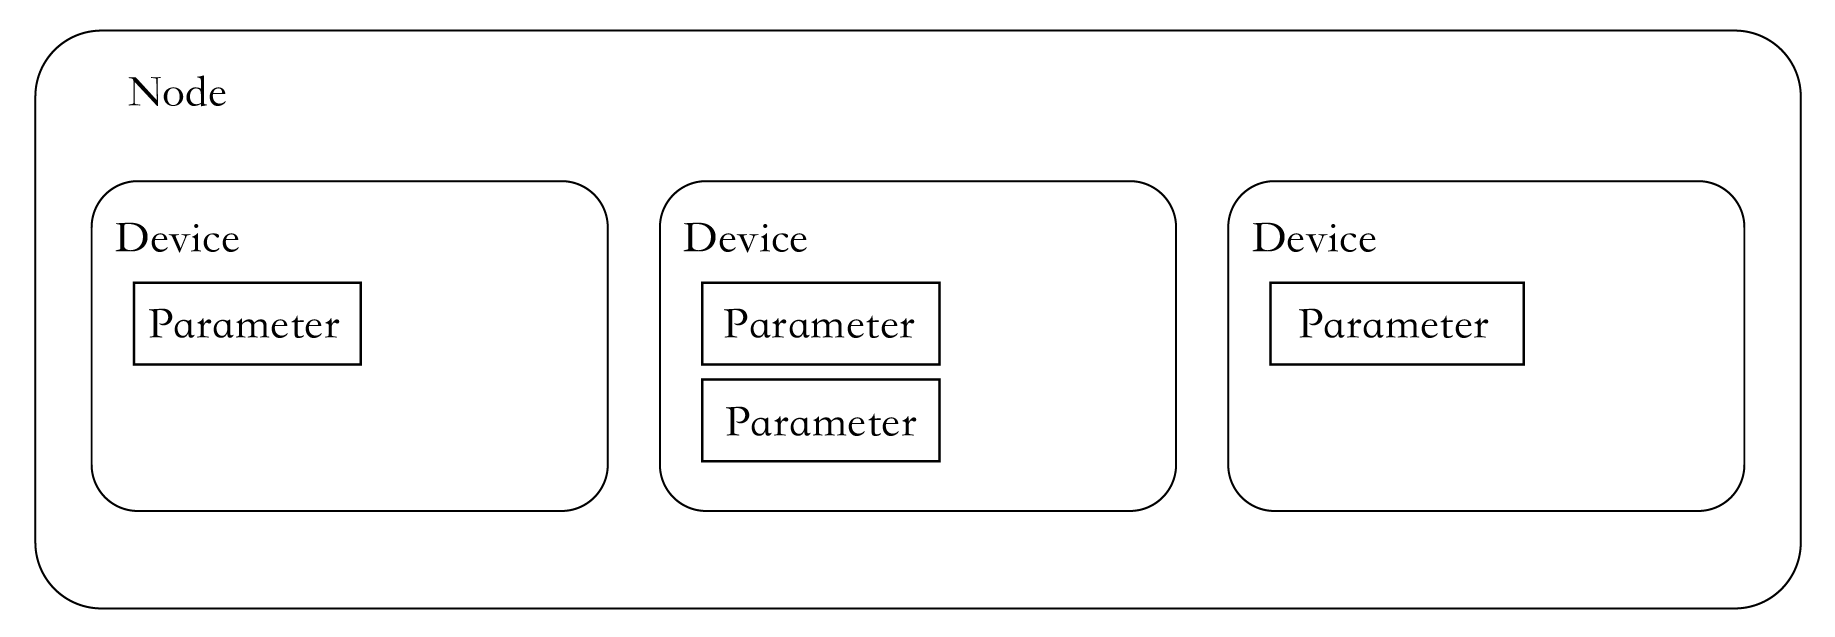
\includegraphics[width=0.65\textwidth]{D9Z/9-6}
    \caption{ESP RainMaker framework}
\end{figure}

\begin{term}{Node}
    It refers to the device model that represents the physical device (such as ESP32-C3) in the cloud. Each node has a unique identifier, namely, node ID. It is the smallest operational unit and a representation of the physical device in the ESP RainMaker framework.
\end{term}

\begin{term}{Node attribute}
    It is used to better describe and define the functions of nodes. ESP RainMaker has set default metadata for the node, including \verb|fw_version| and \verb|model|. The name and type that are set when a node is created also belong to the default metadata. You can also add your own information to the metadata to better describe the node.
\end{term}

\begin{term}{Device}
    It is a logical entity that the user can control, such as a switch, smart light, temperature sensor, or fan. Unlike a node, a device is the smallest unit that can be operated at the user level.
\end{term}

\begin{term}{Device attribute}
    Similar to node attribute, it is used to better describe and define functions of devices.
\end{term}

\begin{term}{Service}
    In the ESP RainMaker framework, a service is a very similar entity to a device. The main difference is that the service does not require operations from the user. For example, the OTA upgrade service has some states that do not require any operation and management from the user.
\end{term}

\begin{term}{Parameter}
    It is used to implement functions of devices and services, such as the power status, brightness, and colour of a smart light, and status updates during OTA upgrades.
\end{term}

The concepts of nodes, devices, parameters, and services in the ESP RainMaker framework can aptly describe the form and functions of the product. For example, to create a smart light with controllable power status, brightness, colour, and scheduled switching, the light is represented by a node and a device, the power status, brightness, and colour are controlled by parameters, and the scheduling function is achieved by a service.

\subsection{Node and Cloud Backend Communication Protocol}
The communication between the node and cloud backend is encrypted using TLS over MQTT, and their identities are mutually authenticated using X.509 certificates. The private key used for the node connection is automatically generated on the node.

During the first Wi-Fi provisioning, ESP32-C3 obtains a certificate through Assisted Claiming, and saves it in its flash. The process for ESP32-C3 to use Assisted Claiming is shown in Figure 9.7.

\begin{figure}[!h]
    \centering
    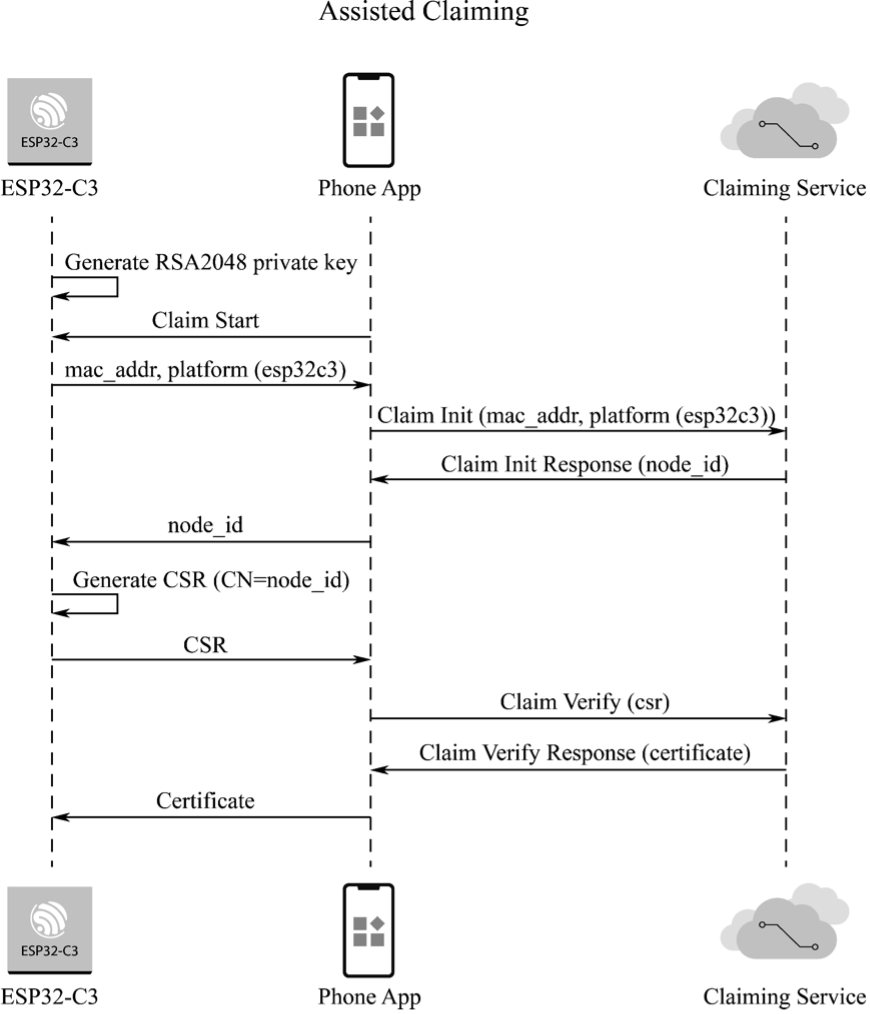
\includegraphics[width=0.65\textwidth]{D9Z/9-7}
    \caption{ESP32-C3 Assisted Claiming}
\end{figure}

\begin{enumerate}[label=(\arabic*)]
    \item ESP32-C3 generates an RSA2048 private key, uses its MAC address as the initial node ID, and then sends relevant messages to the smartphone app.
    \item During the first provisioning, the app and the Claiming Service authenticate each other’s identity. Once the authentication is successful, the receiving server issues a node ID, which is then forwarded by the app to ESP32-C3.
    \item ESP32-C3 generates a CSR with the CN field set as the node ID. Then, the CSR is forwarded by the app to the Claiming Service.
    \item The Claiming Service verifies the CSR and issues the certificate, which is then forwarded by the app to ESP32-C3.
\end{enumerate}

The node ID serves not only as a means of identifying a node during certificate application but also as a way to map to a user and filter MQTT messages. For example, a node can only subscribe to topics with a specific prefix (\verb|node/<node_id>/*|) and publish messages to those topics.

ESP RainMaker defines some default messages, including configuration messages, control messages, status messages, initial status messages, mapping messages, OTA upgrade messages, and warning messages. These messages are packaged in JSON and sent to the cloud backend over MQTT.

The configuration message is published by nodes through \verb|node/<node_id>/config|. It contains information about the node itself, its attributes, devices, device attributes, services, and parameters. Here is an example.

\begin{codebloc}
\begin{tabular}{d}
\vspace{2pt}
\begin{verbatim}
1.  //Configuration message for led_light
2.  {
3.      "node_id": "xxxxxxxxxx",                    //Node ID
4.      "config_version": "2020-03-20",             //Configuration version
5.      "info": {                                   //Node information
6.          "name": "ESP RainMaker Device",
7.          "fw_version": "1.0",
8.          "type": "Lightbulb",
9.          "model": "led_light"
10.     },
11.     "devices": [                                //Devices of this node
12.         {
13.             "name": "Light",
14.             "type": "esp.device.lightbulb",
15.             "primary": "Power",
16.             "params": [                         //Device parameters
17.             {
18.                 "name": "Name",
19.                 "type": "esp.param.name",
20.                 "data_type": "string",
21.                 "properties": ["read", "write"]
22.             },
23.             {
24.                 "name": "Power",
25.                 "type": "esp.param.power",
26.                 "data_type": "bool",
27.                 "properties": ["read", "write"],
28.                 "ui_type": "esp.ui.toggle"
29.             },
30.             ......
31.             ]
32.         }
33.         ],
34.         "services": [                       		//Node services
35.         {
36.             "name": "OTA",
37.             "type": "esp.service.ota",
\end{verbatim}
\verb|38.             "params": [|
\end{tabular}
\end{codebloc}

\begin{codebloc}
\begin{tabular}{d}
\vspace{2pt}
\begin{verbatim}
39.             {
40.                 "name": "Status",
41.                 "type": "esp.param.ota_status",
42.                 "data_type": "string",
43.                 "properties": ["read"]
44.             }
45.             ......
46.             ]
47.         }
48.     ]
\end{verbatim}
\verb|49. }|
\end{tabular}
\end{codebloc}

The smartphone app can obtain the unique identifier of the product by parsing \verb|node_id|, the device information and number by parsing \verb|devices|, the services by parsing the \verb|services|, and the read and write permissions of the app by parsing \verb|properties|. If \verb|ui_type| of \verb|params| in \verb|devices| is set, the app will display the corresponding UI. For more information on the use of standard parameters, standard devices, and standard UI, please refer to Section 9.4.7.

The downlink control message is used the app and third-party applications to control nodes. It contains device parameters that need to be updated. To receive such messages, a node needs to subscribe to the topic \verb|node/<node_id>/remote|. Here is an example of control messages.

\begin{codebloc}
\begin{tabular}{d}
\vspace{2pt}
\begin{verbatim}
1.  {
2.      "Light": {
3.          "Power": false
4.      }
\end{verbatim}
\verb|5.  }|
\end{tabular}
\end{codebloc}

A node can actively report its status messages through the topic \verb|node/<node_id>/params|\\ \verb|/local|. The cloud backend will cache the parameters in the message and push them to the clients that have enabled the push function.

The mapping message is used to map nodes to users. An unmapped node needs to be mapped to a user first to ensure that only that user has access to it. The mapping request occurs during the Wi-Fi configuration phase. During Wi-Fi provisioning, the device receives the user ID and security key from the smartphone. Once the node is connected to the cloud backend, it will concatenate the user ID and security key with its own node ID and send them to the cloud backend. Here is an example of mapping messages.

\begin{codebloc}
\begin{tabular}{d}
\vspace{2pt}
\begin{verbatim}
1.  {
2.      "node_id": "112233AABBCC",
3.      "user_id": "02e95749-8d9d-4b8e-972c-43325ad27c63",
4.      "secret_key": "9140ef1d-72be-48d5-a6a1-455a27d77dee"
\end{verbatim}
\verb|5.  }|
\end{tabular}
\end{codebloc}

After receiving the above message, the cloud backend will check whether it receives the same security key from the app. If yes, it will map the user to the device. The mapping process is shown in Figure 9.8.

\begin{figure}[!h]
    \centering
    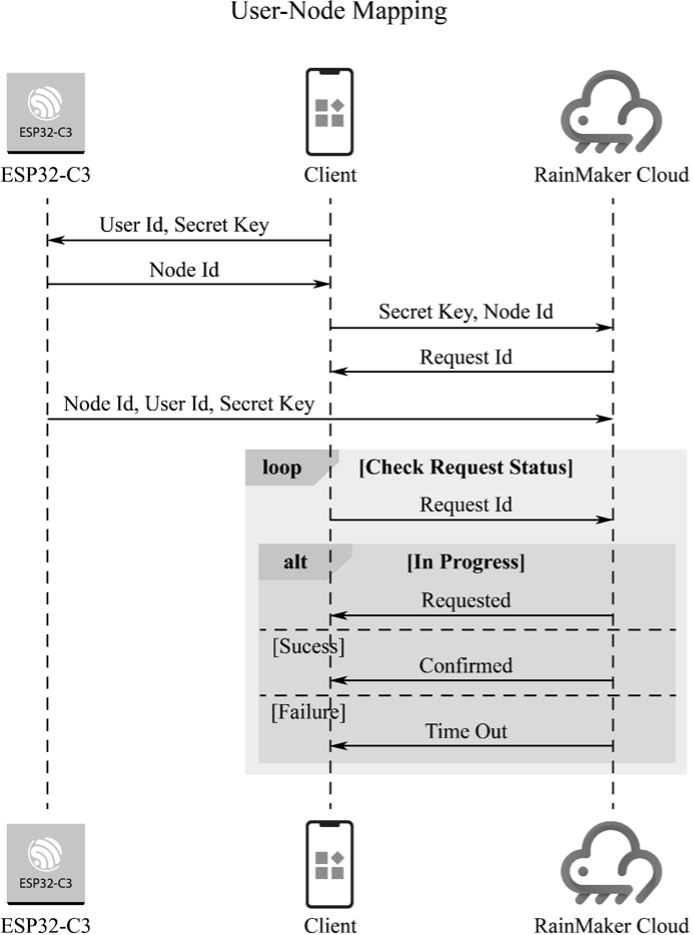
\includegraphics[width=0.6\textwidth]{D9Z/9-8}
    \caption{Mapping process}
\end{figure}

The OTA upgrade message is used to implement OTA upgrades for nodes. It uses three MQTT topics: \verb|node/<node_id>/otafetch|, \verb|node/<node_id>/status|, and \verb|node/<node_|\\ \verb|id>/otaurl|. These topics respectively report OTA upgrade status, distribute OTA upgrade firmware, and query OTA upgrade tasks. The code is as follows:

\begin{codebloc}
\begin{tabular}{d}
\vspace{2pt}
\begin{verbatim}
1.  //Distribute OTA upgrade firmware
2.  {
3.      "url": "<ota_image_url>",
4.      "ota_job_id": "<ota_job_id>",
5.      "file_size": "<num_bytes>"
6.  }
7.
8.  //Query OTA upgrade tasks
\end{verbatim}
\verb|9.  {|
\end{tabular}
\end{codebloc}

\begin{codebloc}
\begin{tabular}{d}
\vspace{2pt}
\begin{verbatim}
10.     "node_id": "<node_id>",
11.     "fw_version": "<fw_version>"
12. }
13.
14. //Report OTA upgrade status
15. {
16.     "ota_job_id": "<ota_job_id>",
17.     "status": "<in-progress/success/fail>",
18.     "additional_info": "<additional_info>"
\end{verbatim}
\verb|19. }|
\end{tabular}
\end{codebloc}

The warning message is a type of push messages used to notify and remind users. A node can publish warning messages via the topic \verb|node/<node_id>/alert|. After receiving a warning message, the app pushes it to the smartphone notification bar. All the data in the cloud backend have push properties, and the use of this topic explicitly marks the data as a notification that needs to be actively pushed to the smartphone’s notification bar. Here is an example of warning messages.

\begin{codebloc}
\begin{tabular}{d}
1.  {

2.      "esp.alert.str": "alert"

3.  }
\end{tabular}
\end{codebloc}

\subsection{Communication between Client and Cloud Backend}
ESP RainMaker offers two client tools: app and CLI, both of which are implemented using the RESTful API. This section briefly explains how to use the CLI tool that comes with the device SDK to communicate with the cloud backend.

The CLI tool is a Python-based submodule of the esp-rainmaker repository, under the \verb|esp-|\\ \verb|rainmaker/cli| directory. To use it, please refer to Chapter 4 to set up the ESP-IDF environment and export the ESP-IDF environment variables. You can verify whether the ESP-IDF and Python environments are ready by running the following commands:

\begin{codebloc}
\begin{tabular}{d}
\# Print ESP-IDF version\newline
\$ \textbf{idf.py --version}\newline
ESP-IDF v4.3.2\newline
\vspace{10pt}
\# Print Python version\newline
\$ \textbf{python3 --version}\newline
Python 3.6.9
\end{tabular}
\end{codebloc}

A similar Shell output to the above indicates that the ESP-IDF environment is ready. Note that the CLI tool depends on Python 3.x, and the older versions need upgrading.

After the ESP-IDF environment is ready, use pip to install the Python dependencies of the CLI tool with the following commands:

\begin{codebloc}
\begin{tabular}{d}
\$ \textbf{cd {your RainMaker path}/esp-rainmaker/cli}\newline
\$ \textbf{pip install -r requirements.txt}
\end{tabular}
\end{codebloc}

\begin{codebloc}
\begin{tabular}{d}
\vspace{2pt}
\begin{verbatim}
Collecting argparse
  Using cached argparse-1.4.0-py2.py3-none-any.whl (23 kB)
...
...
...
Installing collected packages: cryptography, argparse
  Attempting uninstall: cryptography
    Found existing installation: cryptography 2.9.2
    Uninstalling cryptography-2.9.2:
      Successfully uninstalled cryptography-2.9.2
Successfully installed argparse-1.4.0 cryptography-2.4.2
\end{verbatim}
\verb|WARNING: You are using pip version 21.1.2; however, version 21.3.1 is available.|
\end{tabular}
\end{codebloc}

Once the environment is set up, you can use the CLI tool to communicate with the cloud backend. All the commands supported by the CLI are listed in Table 9.4, and you can view the usage of each command by running \verb|python3 rainmaker.py –h|. Additionally, you can use the parameter \verb|-h| together with each command to view more help information.

\begin{table}[h!]
    \renewcommand{\arraystretch}{1.15}
    \caption{CLI commands}
    \begin{tabular}{|>{\ttfamily\small}m{8em}|m{31em}|}
        \hline
        \rowcolor{LightBlue} \multicolumn{1}{|c|}{\textbf{Command}}&\multicolumn{1}{c|}{\textbf{Description}}\\
        \hline
        signup&Sign up for ESP RainMaker\\
        \hline
        login&Login to ESP RainMaker\\
        \hline
        logout&Logout current (logged-in) user\\
        \hline
        forgotpassword&Reset the password\\
        \hline
        getnodes&List all nodes associated with the user\\
        \hline
        getnodeconfig&Get node configuration\\
        \hline
        getnodestatus&Get online/offline status of the node\\
        \hline
        setparams&Set node parameters\\
        \hline
        getparams&Get the last parameter of the node in the cloud\\
        \hline
        removenode&Remove user node mapping\\
        \hline
        provision&Provision the node to join Wi-Fi network\\
        \hline
        getmqtthost&Get the address of the MQTT host that the node connects to\\
        \hline
        claim&Perform host driven claimming to the node and get the MQTT cerficate\\
        \hline
        test&Test whether the node has been mapped to the user\\
        \hline
        otaupgrade&Distribute OTA upgrade information\\
        \hline
        getuserinfo&Get detailed information of the logged-in user\\
        \hline
        sharing&Share the node\\
        \hline
    \end{tabular}
\end{table}

The claim command in the CLI tool is for host driven claiming, which is no longer supported in ESP32-C3. Instead, the more convenient Self Claiming is supported in ESP32-C3.

Before using any other command, you need to first run the \verb|signup| command to sign up for an ESP RainMaker account:

\begin{codebloc}
\begin{tabular}{d}
\$ \textbf{cd {your RainMaker path}/esp-rainmaker/cli}

\$ \textbf{cd python3 rainmaker.py signup someone@example.com}
\begin{verbatim}
Choose a password
Password :
Confirm Password :
Enter verification code sent on your Email.
Verification Code : 973854
Signup Successful
\end{verbatim}
\verb|Please login to continue with ESP Rainmaker CLI|
\end{tabular}
\end{codebloc}

Check the verification code in your email, as shown in Figure 9.9.

\begin{figure}[!h]
    \centering
    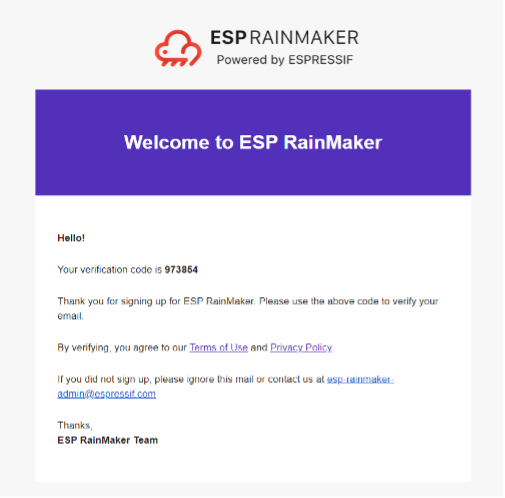
\includegraphics[width=0.7\textwidth,frame]{D9Z/9-9}
    \caption{Verification code in email}
\end{figure}

Then, log in.

Execute the \verb|login| command, and the Shell will open a web page, as shown in Figure 9.10. Enter your account and password in the box.

\begin{figure}[!h]
    \centering
    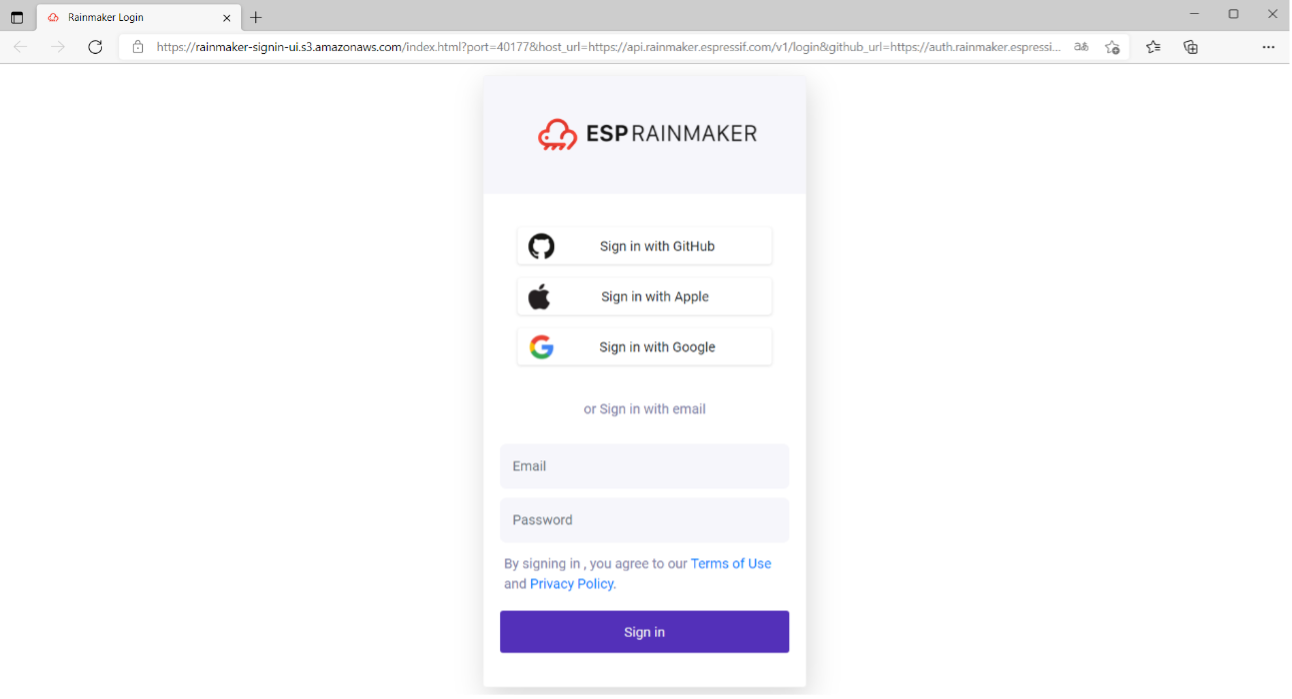
\includegraphics[width=0.9\textwidth,frame]{D9Z/9-10}
    \caption{Log in to ESP RainMaker using web browser}
\end{figure}

Alternatively, you can enter the command \verb|login| together with the parameter \verb|-email| to directly log in using CLI:

\begin{codebloc}
\begin{tabular}{d}
\$ \textbf{python3 rainmaker.py login --email someone@example.com}

Password:

Login Successful
\end{tabular}
\end{codebloc}

\subsection{User Roles}
As mentioned earlier, user-node mapping aims to ensure that each node is controlled by a unique user. There are two types of users in ESP RainMaker: admin users and end users.

\begin{term}{Admin user: }
    a user who owns the MQTT certificate of a given node or gets the certificate through claiming service. Admin users can access nodes via the ESP RainMaker dashboard, push OTA firmware updates, and use ESP Insight for remote monitoring, but cannot read or write node parameters.
\end{term}

\begin{term}{End user:}
    a user who has the control permissions to a given node. End users can set and obtain node parameters and configuration but cannot view nodes via the ESP RainMaker dashboard. They are subdivided into primary users and secondary users.

    \parskip 6pt
    \begin{secterm}{Primary user:}
        a user who last performs the user-node mapping. Primary users can access node configuration, read/write node parameters, and add/remove/view other secondary users.
    \end{secterm}

    \begin{secterm}{Secondary user:}
        any user who gets access to a node via node sharing. Secondary users can access node configuration and read/write node parameters, but cannot add/remove/view other secondary users.
    \end{secterm}
\end{term}

\subsection{Basic Services}
ESP RainMaker services are practical examples that integrate specific functions to facilitate secondary development and enrich the functionality of nodes. For example, the scheduling service provides devices with the offline timing/countdown function; the system service offers the remote reboot and factory reset functions; the time \& time zone service enables the time zone switching function; the OTA upgrade service provides the remote update function; and the local control service allows fast, stable, and secure LAN communication. These services can be quickly implemented with simple configuration.

\textbf{1.	Time \& time zone service}

Fetching time is one of the most critical tasks for an IoT device after connecting to the Internet, especially when the scheduling service is enabled. In ESP RainMaker, there are two important concepts: time and time zone.

Time is typically fetched using Simple Network Time Protocol (SNTP). The ESP RainMaker SDK provides an abstraction layer over the SNTP component in ESP-IDF, making it easy for you to synchronise and check time. The code is as follows:

\begin{codebloc}
\begin{tabular}{d}
\vspace{2pt}
\fontsize{9pt}{10pt}\selectfont
\begin{verbatim}
1. /*Initialise time synchronisation. This will call the SNTP component internally and 
2. set the SNTP server through sntp_server_name passed by esp_rmaker_time_config_t*/
3. esp_err_t esp_rmaker_time_sync_init(esp_rmaker_time_config_t *config);
4.
5. //Check if time has been synchronised by comparison with the standard time 1546300800
6. bool esp_rmaker_time_check(void);
7.
8. //Wait for time to be synchronised
\end{verbatim}
\verb|9. esp_err_t esp_rmaker_time_wait_for_sync(uint32_t ticks_to_wait);|
\end{tabular}
\end{codebloc}

As countries and regions in different longitudes have different local times and time zones, the \verb|TZ| environment variable and the \verb|tz_set()| function are provided by ESP-IDF to set the time zone. RainMaker provides an abstraction layer over this and provides multiple ways of setting it. For example:

(1) Using the \textbf{C API}.

\begin{codebloc}
\begin{tabular}{d}
\vspace{2pt}
\begin{verbatim}
1.  //Set time zone using the timezone region string
2.  esp_err_t esp_rmaker_time_set_timezone(const char *tz);
3.
4.  //Set time zone using the POSIX format
\end{verbatim}
\verb|5.  esp_err_t esp_rmaker_time_set_timezone_posix(const char *tz_posix);|
\end{tabular}
\end{codebloc}

(2) Modifying \verb|Default Timezone| in \verb|menuconfig|. To use this method, you need to have some basic understanding of ESP-IDF. For more information, please refer to Chapter 4. The configuration for this method is as follows:

\begin{codebloc}
\begin{tabular}{d}
\vspace{2pt}
\begin{verbatim}
 (Top) → Component config → ESP RainMaker Common
    Espressif IoT Development Framework Configuration
…
(Asia/Shanghai) Default Timezone
\end{verbatim}
\verb|…|
\end{tabular}
\end{codebloc}

(3) Setting time zone directly on the \textbf{client side} via the time zone service. To enable this service, call the following function on the device side:

\begin{codebloc}
\begin{tabular}{d}
\verb|1.  esp_err_t esp_rmaker_timezone_service_enable(void);|
\end{tabular}
\end{codebloc}

\textbf{2.	Scheduling service}

The scheduling service performs periodic modifications to device parameters. For example, if you need to turn on a light at 7pm and turn it off at 11pm every day, this service can spare you from manually turning it on and off. After configured, this service runs independently on the device and does not rely on the network, which means that the device can perform the configured operation correctly even when the device is disconnected from the network. To enable this service, call the following function on the device side:

\begin{codebloc}
\begin{tabular}{d}
\verb|1.  esp_err_t esp_rmaker_schedule_enable(void);|
\end{tabular}
\end{codebloc}

\textbf{3.	OTA upgrade service}

ESP RainMaker provides the OTA upgrade service to update firmware. You only need to call a simple API to enable it. There are two methods of performing OTA upgrade.

(1) \textbf{OTA upgrade using parameters}. This is the simplest way for developers to upgrade firmware OTA. You only need to upload the firmware to any secure web server and provide the URL to the node. This method can be triggered from the ESP RainMaker CLI client. The \verb|otaupgrade| command in the CLI tool is used to complete the upgrade, as shown below:

\begin{codebloc}
\begin{tabular}{d}
\vspace{2pt}
\begin{verbatim}
1.  esp_rmaker_ota_config_t ota_config = {
2.      .server_cert = ESP_RMAKER_OTA_DEFAULT_SERVER_CERT,
3.  };
\end{verbatim}
\verb|4.  esp_rmaker_ota_enable(&ota_config, OTA_USING_PARAMS);|
\end{tabular}
\end{codebloc}

\vspace{6pt}
(2) \textbf{OTA upgrade using MQTT topics}. This is a more advanced method available to admin users to upgrade firmware OTA. They need to upload the firmware to the dashboard and create a task there to enable the OTA upgrade. The device will receive the OTA upgrade URL and report the upgrade progress over MQTT. The code is as follows:

\begin{codebloc}
\begin{tabular}{d}
\vspace{2pt}
\begin{verbatim}
1.  esp_rmaker_ota_config_t ota_config = {
2.      .server_cert = ESP_RMAKER_OTA_DEFAULT_SERVER_CERT,
3.  };
\end{verbatim}
\verb|4.  esp_rmaker_ota_enable(&ota_config, OTA_USING_TOPICS);|
\end{tabular}
\end{codebloc}

\textbf{4.	Local control service}

Besides remote control, ESP RainMaker also enables the client to locally control the nodes that are on the same Wi-Fi network as the client. This makes the entire process of control and response faster and more reliable. ESP-IDF provides a component called ESP Local Control, which uses mDNS-based discovery and HTTP-based control. It is now integrated into the ESP RainMaker SDK. 

Local control does not require adding a service to the node configuration message. It protects data using asymmetric encryption algorithms and transmits the Proof of possession (PoP) to the app through the local control service. The smartphone app completes encryption using the PoP.

\begin{codebloc}
\begin{tabular}{d}
\vspace{2pt}
\begin{verbatim}
# Enable local control
CONFIG_ESP_RMAKER_LOCAL_CTRL_ENABLE=y

# Enable local control encryption
\end{verbatim}
\verb|CONFIG_ESP_RMAKER_LOCAL_CTRL_SECURITY_1=y|
\end{tabular}
\end{codebloc}

\textbf{5.	System service}

ESP RainMaker presets a set of system services for factory reset and remote reboot. Smartphone apps can use these services to erase the network configuration information on the device and unmap users from the devices. To enable this service, call the following API on the device side:

\begin{codebloc}
\begin{tabular}{d}
\fontsize{9pt}{9pt}\selectfont
\verb|1.  esp_err_t esp_rmaker_system_service_enable(esp_rmaker_system_serv_config_t *config)|
\end{tabular}
\end{codebloc}

\subsection{Smart Light Example}
The RainMaker SDK is built on top of ESP-IDF and provides simple APIs for building applications based on the ESP RainMaker specification. This section will explain and run the smart light example. The code is as follows:

\begin{codebloc}
\begin{tabular}{d}
\vspace{2pt}
\begin{verbatim}
1.  esp_rmaker_device_t *light_device;
2.  //Callback function to handle commands received from ESP RainMaker
3.  static esp_err_t write_cb(const esp_rmaker_device_t *device,
4.                            constesp_rmaker_param_t *param,
5.                            const esp_rmaker_param_val_t val,
6.                            void *priv_data,
7.                            esp_rmaker_write_ctx_t *ctx)
8.  {
9.      if (ctx) {
10.         ESP_LOGI(TAG,
11.                 "Received write request via : %s",
12.                 esp_rmaker_device_cb_src_to_str(ctx->src));
13.     }
\end{verbatim}
\verb|14.     const char *device_name = esp_rmaker_device_get_name(device);|
\end{tabular}
\end{codebloc}

\begin{codebloc}
\begin{tabular}{d}
\vspace{2pt}
\begin{verbatim}
15.     const char *param_name = esp_rmaker_param_get_name(param);
16.     if (strcmp(param_name, ESP_RMAKER_DEF_POWER_NAME) == 0) {
17.         ESP_LOGI(TAG,
18.                 "Received value = %s for %s - %s",
19.                 val.val.b? "true" : "false",
20.                 device_name,
21.                 param_name);
22.         app_light_set_power(val.val.b);
23.     } else if (strcmp(param_name, ESP_RMAKER_DEF_BRIGHTNESS_NAME) == 0) {
24.         ESP_LOGI(TAG,
25.                 "Received value = %d for %s - %s",
26.                 val.val.i,
27.                 device_name,
28.                 param_name);
29.         app_light_set_brightness(val.val.i);
30.     } else if (strcmp(param_name, ESP_RMAKER_DEF_HUE_NAME) == 0) {
31.         ESP_LOGI(TAG,
32.                 "Received value = %d for %s - %s",
33.                 val.val.i, 
34.                 device_name, 
35.                 param_name);
36.         app_light_set_hue(val.val.i);
37.     } else if (strcmp(param_name, ESP_RMAKER_DEF_SATURATION_NAME) == 0) {
38.         ESP_LOGI(TAG, 
39.                 "Received value = %d for %s - %s",
40.                 val.val.i, 
41.                 device_name, 
42.                 param_name);
43.         app_light_set_saturation(val.val.i);
44.     } else {
45.         //Omit parameters that do not need processing
46.         return ESP_OK;
47.     }
48.     esp_rmaker_param_update_and_report(param, val);
49.     return ESP_OK;
50. }
51.	
52. void app_main()
53. {
54.     //Initialise the driver layer
55.     app_driver_init();
56.	
57.     //Initialise the NVS partition
58.     esp_err_t err = nvs_flash_init();
59.     if (err == ESP_ERR_NVS_NO_FREE_PAGES || err ==
\end{verbatim}
\verb|60.               ESP_ERR_NVS_NEW_VERSION_FOUND) {|
\end{tabular}
\end{codebloc}

\begin{codebloc}
\begin{tabular}{d}
\vspace{2pt}
\begin{verbatim}
61.         ESP_ERROR_CHECK(nvs_flash_erase());
62.         err = nvs_flash_init();
63.     }
64.     ESP_ERROR_CHECK( err );
65.	
66.     //Initialise Wi-Fi
67.     app_wifi_init();
68.	
69.     //Initialise ESP RainMaker Agent
70.     esp_rmaker_config_t rainmaker_cfg = {
71.         .enable_time_sync = false,
72.     };
73.     esp_rmaker_node_t *node = esp_rmaker_node_init(&rainmaker_cfg,
74.                                                   "ESP RainMakerDevice", 
75.                                                   "Lightbulb");
76.     if (!node) {
77.         ESP_LOGE(TAG, "Could not initialise node. Aborting!!!");
78.         vTaskDelay(5000/portTICK_PERIOD_MS);
79.         abort();
80.     }
81.	
82.     //Create the device and add parameters
83.     light_device = esp_rmaker_lightbulb_device_create("Light",
84.                                                      NULL,
85.                                                      DEFAULT_POWER);
86.     esp_rmaker_device_add_cb(light_device, write_cb, NULL);
87.     esp_rmaker_device_add_param(light_device,
88.                                 esp_rmaker_brightness_param_create(  
89.                                 ESP_RMAKER_DEF_BRIGHTNESS_NAME, 
90.                                 DEFAULT_BRIGHTNESS));
91.     esp_rmaker_device_add_param(light_device, esp_rmaker_hue_param_creat(
92.                                 ESP_RMAKER_DEF_HUE_NAME,  
93.                                 DEFAULT_HUE));
94.     esp_rmaker_device_add_param(light_device, 
95.                                 esp_rmaker_saturation_param_create( 
96.                                 ESP_RMAKER_DEF_SATURATION_NAME, 
97.                                 DEFAULT_SATURATION));
98.     esp_rmaker_node_add_device(node, light_device);
99.	
100.    //Enable OTA upgrade
101.    esp_rmaker_ota_config_t ota_config = {
102.        .server_cert = ota_server_cert,
103.    };
104.    esp_rmaker_ota_enable(&ota_config, OTA_USING_PARAMS);
105.
\end{verbatim}
\verb|106.    //Enable time & time zone service|
\end{tabular}
\end{codebloc}

\begin{codebloc}
\begin{tabular}{d}
\vspace{2pt}
\begin{verbatim}
107.    esp_rmaker_timezone_service_enable();
108.
109.    //Enable scheduling service
110.    esp_rmaker_schedule_enable();
111.
112.    //Enable ESP Insight
113.    app_insights_enable();
114.
115.    //Enable ESP RainMaker Agent
116.    esp_rmaker_start();
117.
118.    //Enable Wi-Fi
119.    err = app_wifi_start(POP_TYPE_RANDOM);
120.    if (err != ESP_OK) {
121.        ESP_LOGE(TAG, "Could not start Wifi. Aborting!!!");
122.        vTaskDelay(5000/portTICK_PERIOD_MS);
123.        abort();
124.    }
\end{verbatim}
\verb|125.}|
\end{tabular}
\end{codebloc}

Firstly, the above example initialises the hardware driver by configuring GPIO and initialising peripherals. Next, the NVS partition is initialised in preparation for reading data from the flash. The partition table \verb|partitions.csv| is as follows:

\begin{codebloc}
\begin{tabular}{d}
\vspace{2pt}
\begin{verbatim}
1.  # Name,   Type, SubType, Offset,    Size,   Flags
2.  # Note: Firmware partition offset needs to be 64K aligned, initial 36K (9 
3.  sectors) are reserved for bootloader and partition table
4.  sec_cert, 0x3F, ,       0xd000,     0x3000, ,
5.  nvs,      data, nvs,    0x10000,    0x6000,
6.  otadata,  data, ota,    ,           0x2000
7.  phy_init, data, phy,    ,           0x1000,
8.  ota_0,    app,  ota_0,  0x20000,    1600K,
9.  ota_1,    app,  ota_1,  ,           1600K,
\end{verbatim}
\verb|10. fctry,    data, nvs,    0x340000,   0x6000|
\end{tabular}
\end{codebloc}

As shown in the above partition table, there are two NVS partitions in this example project: \verb|nvs| and \verb|fctry|. The former is used to store network configuration and local scheduling information and the latter is used to store certificate information.

Then, Wi-Fi is initialised. This step must be performed before the \verb|esp_rmaker_node_|\\ \verb|init()| function is called. If the \verb|fctry| partition does not contain a certificate, Assisted Claiming will be enabled because the MAC address can be used as the initial node ID when Wi-Fi is initialised. Afterward, the device model is created and the callback function is added. All cloud downlink data will be transmitted through this callback function, and the ESP RainMaker core task is started. Finally, Wi-Fi is enabled. If the device has not been connected to Wi-Fi, the provisioning application will be automatically started. The application is implemented using the \verb|wifi_provisioning| component in ESP-IDF and started by calling \verb|app_wifi_start()| in the ESP RainMaker SDK.

Run \verb|idf.py| to compile and flash the \verb|led_light| project and \verb|idf.py monitor| to open the monitor, and then you will see the following log:

\begin{codebloc}
\begin{tabular}{d}
\vspace{2pt}
\begin{verbatim}
I (30) boot: ESP-IDF v4.3.2-dirty 2nd stage bootloader
...
...
...
I (488) cpu_start: Starting scheduler.
I (493) gpio: GPIO[9]| InputEn: 1| OutputEn: 0| OpenDrain: 0| Pullup: 1| 
Pulldown: 0| Intr:3
I (503) coexist: coexist rom version 9387209
I (503) pp: pp rom version: 9387209
I (503) net80211: net80211 rom version: 9387209
I (523) wifi:wifi driver task: 3fca4d8c, prio:23, stack:6656, core=0
I (523) system_api: Base MAC address is not set
I (523) system_api: read default base MAC address from EFUSE
...
...
...
I (623) esp_rmaker_work_queue: Work Queue created.
I (623) esp_claim: Initialising Assisted Claiming. This may take time.
W (633) esp_claim: Generating the private key. This may take time.
I (110533) esp_rmaker_node: Node ID ----- 7CDFA161BE38
I (21213) esp_rmaker_node: Node ID ----- 7CDFA1C21DA0
I (21213) esp_rmaker_ota: OTA state = 2
I (21213) esp_rmaker_ota_using_params: OTA enabled with Params
I (21223) esp_rmaker_time_service: Time service enabled
\end{verbatim}
I (21223) \fontsize{9.5pt}{10pt}\selectfont\verb|esp_rmaker_time: Initializing SNTP. Using the SNTP server: pool.ntp.org|
\footnotesize
\begin{verbatim}
I (21233) app_insights: Enable CONFIG_ESP_INSIGHTS_ENABLED to get Insights.
I (21243) esp_rmaker_core: Starting RainMaker Work Queue task
I (21253) esp_rmaker_work_queue: RainMaker Work Queue task started.
I (21253) esp_claim: Waiting for assisted claim to finish.
...
...
...
\end{verbatim}
\vspace{5pt}

\includegraphics[width=0.2\textwidth]{D9Z/9-4-6}

I (21623) \fontsize{9pt}{10pt}\selectfont\verb|app_wifi: If QR code is not visible, copy paste the below URL in a browser.|
\footnotesize
\verb|https://rainmaker.espressif.com/qrcode.html?data={"ver":"v1","name":"PROV_8a20|
\verb|e0","pop":"827e49ae","transport":"ble"}|

\verb|I (21633) app_wifi: Provisioning Started. Name : PROV_8a20e0, POP : 827e49ae|
\end{tabular}
\end{codebloc}

Use the smartphone app to scan the QR code. If no certificate is present in the \verb|fctry| partition, Assisted Claiming will be enabled, as shown in Figure 9.11.

\begin{figure}[!h]
    \centering
    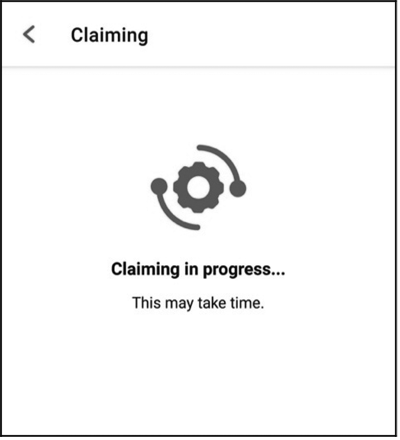
\includegraphics[width=0.4\textwidth]{D9Z/9-11}
    \caption{Interface for enabling Assisted Claiming}
\end{figure}

\begin{codebloc}
\begin{tabular}{d}
\vspace{2pt}
\begin{verbatim}
...
...
I (444493) esp_claim: Assisted Claiming Started.
I (447603) esp_rmaker_core: New Node ID ----- nq8xT6p53BZHTm6k8AZqN
\end{verbatim}
\verb|I (472813) esp_claim: Assisted Claiming was Successful.|
\end{tabular}
\end{codebloc}

After the certificate is obtained, the device enters the network configuration phase. The smartphone app will send the selected SSID and password to the device, which will then attempt to connect to the router and the cloud, as shown in Figure 9.12.

\begin{codebloc}
\begin{tabular}{d}
\vspace{2pt}
\begin{verbatim}
...
...
I (491113) esp_rmaker_user_mapping: Received request for node details
I (491113) esp_rmaker_user_mapping: Got user_id = 764865be-e49f-49d1-afa1-696d6
a7e3233, secret_key = a3c89473-514f-4aa4-a190-a9aa38e7a9d8
I (491123) esp_rmaker_user_mapping: Sending status SUCCESS
I (491753) app_wifi: Received Wi-Fi credentials
        SSID     : Xiaomi_32BD
        Password : 12345678
I (495173) wifi:new:<11,0>, old:<1,0>, ap:<255,255>, sta:<11,0>, prof:1
I (495753) wifi:state: init -> auth (b0)
I (495793) wifi:state: auth -> assoc (0)
I (495833) wifi:state: assoc -> run (10)
I (495973) wifi:connected with Xiaomi_32BD, aid = 2, channel 11, BW20, bssid = 
88:c3:97:9e:32:be
I (495973) wifi:security: WPA2-PSK, phy: bgn, rssi: -25
I (495983) wifi:pm start, type: 1
\end{verbatim}
\verb||
\end{tabular}
\end{codebloc}

\begin{codebloc}
\begin{tabular}{d}
\vspace{2pt}
\begin{verbatim}
I (495983) wifi:set rx beacon pti, rx_bcn_pti: 14, bcn_timeout: 14, mt_pti: 
25000, mt_time: 10000
I (496043) wifi:BcnInt:102400, DTIM:1
\end{verbatim}
W (496573) \fontsize{9.5pt}{10pt}\selectfont\verb|wifi:<ba-add>idx:0 (ifx:0, 88:c3:97:9e:32:be), tid:0, ssn:2, winSize:64|
\footnotesize
\begin{verbatim}
I (497503) app_wifi: Connected with IP Address:192.168.31.65
I (497503) esp_netif_handlers: sta ip: 192.168.31.65, mask: 255.255.255.0, gw: 
192.168.31.1
I (497503) wifi_prov_mgr: STA Got IP
I (497503) app_wifi: Provisioning successful
I (497513) esp_mqtt_glue: Initialising MQTT
\end{verbatim}
\verb|I (500973) esp_mqtt_glue: MQTT Connected|
\end{tabular}
\end{codebloc}

After completing the configuration and successfully connecting to the cloud, the device will send a user-node association message, and the app will continue to check the association status, as shown in Figure 9.13.

\begin{figure}[!h]
  \Centering
  \begin{minipage}[b]{0.45\textwidth}
    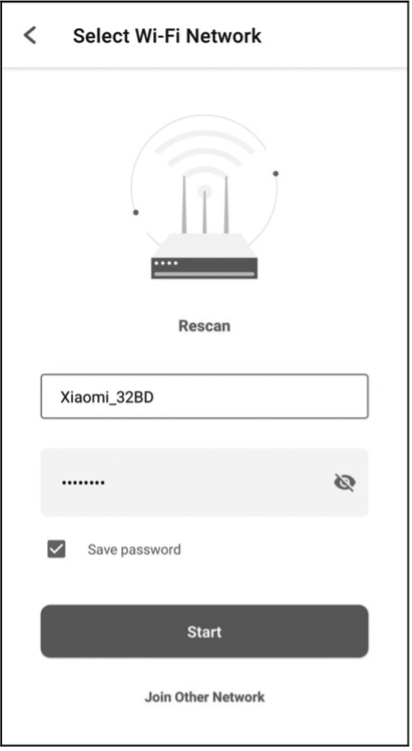
\includegraphics[height=1.5\textwidth]{D9Z/9-12}
    \caption{\Centering\newline Device connecting to router and cloud}
  \end{minipage}
  \begin{minipage}[b]{0.45\textwidth}
    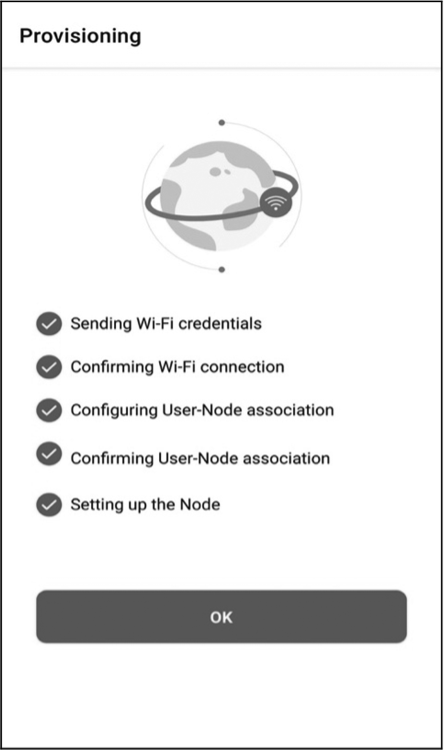
\includegraphics[height=1.5\textwidth]{D9Z/9-13}
    \caption{\Centering\newline Checking association status}
  \end{minipage}
\end{figure}

\begin{codebloc}
\begin{tabular}{d}
\fontsize{10.5pt}{10.5pt}\selectfont
\verb|I (45959) esp_rmaker_user_mapping: User Node association message published |

successfully.
\end{tabular}
\end{codebloc}

After the association, you can check this node using CLI.

\subsection{RainMaker App and Third-Party Integrations}
In Section 9.4.6, we have completed the device provisioning and user-node mapping, enabling control of a smart light through the app. As a result, the smart light icon and UI interface are now displayed on the app’s homepage. The standard parameters, devices, and UIs mentioned earlier are defined by ESP RainMaker and form the basis of its standard framework. By using this framework, the app can accurately manage each device’s parameters and supported services. These standard items, which are listed in the tables below, are also applicable to third-party platforms.

\begin{enumerate}[label=\textbf{(\arabic*)}]
    \item \textbf{Standard UI device types}

    {\renewcommand{\arraystretch}{1.4}
    \fontsize{9pt}{12pt}\selectfont
    \begin{longtable}{|>{\RaggedRight}m{0.11\textwidth}|m{0.2\textwidth}|>{\RaggedRight}m{0.15\textwidth}|m{0.12\textwidth}|m{0.21\textwidth}|>{\Centering}m{0.13\textwidth}|}
        \caption{Standard UI device types \label{9.5}} \\
        \hline
        \rowcolor{LightBlue}\multicolumn{1}{|c|}{\textbf{Name}}&\multicolumn{1}{c|}{\textbf{Type}}&\multicolumn{1}{c|}{\textbf{Params}}&\multicolumn{1}{c|}{\textbf{GVA}}&\multicolumn{1}{c|}{\textbf{Alexa}}&\textbf{Image}\\
        \hline
        \endfirsthead
    
        \multicolumn{6}{r}{Continuation of Table \ref{9.5}}\\
        \hline
        \rowcolor{LightBlue}\multicolumn{1}{|c|}{\textbf{Name}}&\multicolumn{1}{c|}{\textbf{Type}}&\multicolumn{1}{c|}{\textbf{Params}}&\multicolumn{1}{c|}{\textbf{GVA}}&\multicolumn{1}{c|}{\textbf{Alexa}}&\multicolumn{1}{c|}{\textbf{Image}}\\
        \hline
        \endhead
    
        Switch&esp.device.switch&Name, Power*&SWITCH&SWITCH&
\includegraphics[width=0.08\textwidth]{D9Z/switch}\\
        \hline
        Lightbulb&esp.device.lightbulb&Name, Power*, Brightness, Color Temperature, Hue, Saturation, Intensity&LIGHT&LIGHT&
\includegraphics[width=0.08\textwidth]{D9Z/lightbulb}\\
        \hline
        Light&esp.device.light&Name, Power*, Brightness, Color Temperature, Hue, Saturation, Intensity&LIGHT&LIGHT&—\\
        \hline
        Fan&esp.device.fan&Name, Power*, Speed, Direction&FAN&FAN&
\includegraphics[width=0.08\textwidth]{D9Z/fan}\\
        \hline
        Temperature Sensor&esp.device.temperature-sensor&Name, Temperature*&—&TEMPERATURE\_SENSOR&
\includegraphics[width=0.08\textwidth]{D9Z/temp}\\
        \hline
        Outlet&esp.device.outlet&Name, Power&OUTLET&SMARTPLUG&
\includegraphics[width=0.08\textwidth]{D9Z/outlet}\\
        \hline
        Plug&esp.device.plug&Name, Power&OUTLET&SMARTPLUG&—\\
        \hline
        Socket&esp.device.socket&Name, Power&OUTLET&SMARTPLUG&—\\
        \hline
        Lock&esp.device.lock&Name, Lock State&LOCK&SMARTLOCK&
\includegraphics[width=0.08\textwidth]{D9Z/lock}\\
        \hline
        Internal Blinds&esp.device.blinds-internal&Name&BLINDS&INTERIOR\_BLIND&—\\
        \hline
        External Blinds&esp.device.blinds-externa&Name&BLINDS&EXTERIOR\_BLIND&—\\
        \hline
        Garage Door&esp.device.garage-door&Name&GARAGE&GARAGE\_DOOR&—\\
        \hline
        Garage Lock&esp.device.garage-door-lock&Name&GARAGE&SMARTLOCK&—\\
        \hline
        Speaker&esp.device.speaker&Name&SPEAKER&SPEAKER&—\\
        \hline
        Air \newline Conditioner&esp.device.air-conditioner&Name&AC\_UNIT&AIR\_CONDITIONER&—\\
        \hline
        Thermostat&esp.device.thermostat&Name&THERMOSTAT&THERMOSTAT&
\includegraphics[width=0.08\textwidth]{D9Z/thermo}\\
        \hline
        TV&esp.device.tv&Name&TV&TV&—\\
        \hline
        Washer&esp.device.washer&Name&WASHER&WASHER&—\\
        \hline
        Other&esp.device.other&—&—&OTHER&
\includegraphics[width=0.08\textwidth]{D9Z/other}\\
        \hline
    \end{longtable}
    }

    \item \textbf{Standard UI types}

    The standard UI type added to a parameter is displayed as the corresponding UI shown in Table 9.6 in the ESP RainMaker app.

    {\renewcommand{\arraystretch}{1.4}
    \fontsize{9pt}{12pt}\selectfont
    \begin{longtable}{|>{\RaggedRight}m{0.15\textwidth}|>{\RaggedRight}m{0.16\textwidth}|m{0.1\textwidth}|>{\RaggedRight}m{0.25\textwidth}|>{\Centering}m{0.27\textwidth}|}
        \caption{Standard UI types \label{9.6}} \\
        \hline
        \rowcolor{LightBlue}\multicolumn{1}{|c|}{\textbf{Name}}&\multicolumn{1}{c|}{\textbf{Type}}&\multicolumn{1}{c|}{\textbf{Data Types}}&\multicolumn{1}{c|}{\textbf{Requirements}}&\textbf{Sample}\\
        \hline
        \endfirsthead
    
        \multicolumn{5}{r}{Continuation of Table \ref{9.6}}\\
        \hline
        \rowcolor{LightBlue}\multicolumn{1}{|c|}{\textbf{Name}}&\multicolumn{1}{c|}{\textbf{Type}}&\multicolumn{1}{c|}{\textbf{Data Types}}&\multicolumn{1}{c|}{\textbf{Requirements}}&\textbf{Sample}\\
        \hline
        \endhead
    
        Text (Default)&esp.ui.text&All&N/A&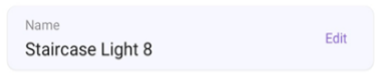
\includegraphics[width=0.27\textwidth]{D9Z/text}\\
        \hline
        Toggle Switch&esp.ui.toggle&bool&N/A&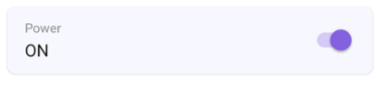
\includegraphics[width=0.27\textwidth]{D9Z/toggle}\\
        \hline
        Slider&esp.ui.slider&int, float&Bounds (min, max)&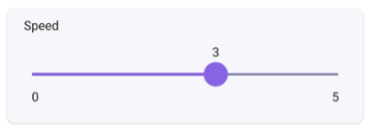
\includegraphics[width=0.27\textwidth]{D9Z/slider}\\
        \hline
        Brightness Slider&esp.ui.slider&int&Param type = esp.param.brightness&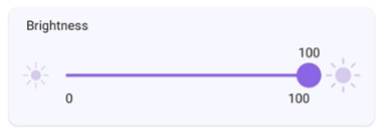
\includegraphics[width=0.27\textwidth]{D9Z/bright}\\
        \hline
        CCT Slider&esp.ui.slider&int&Param type = esp.param.cct&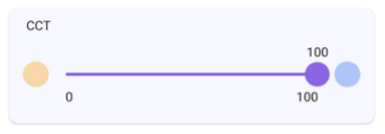
\includegraphics[width=0.27\textwidth]{D9Z/cct}\\
        \hline
        Saturation Slider&esp.ui.slider&int&Param type = esp.param.saturation&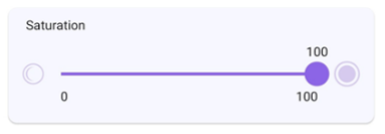
\includegraphics[width=0.27\textwidth]{D9Z/saturation}\\
        \hline		
        Hue Slider&esp.ui.hue-slider&int&Param type = esp.param.hue&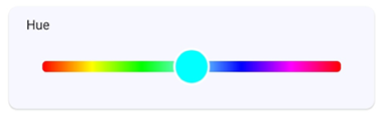
\includegraphics[width=0.27\textwidth]{D9Z/hue}\\
        \hline
        Hue Circle&esp.ui.hue-circle&int&Param type = esp.param.hue&
\includegraphics[width=0.1\textwidth]{D9Z/circle}\\
        \hline
        Push button (Big)&esp.ui.push-btn-big&bool&N/A&
\includegraphics[width=0.11\textwidth]{D9Z/push}\\
        \hline
        Dropdown&esp.ui.dropdown&int/string&Bounds (min/max) for Int\newline Valid strs for String&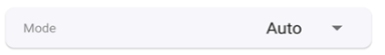
\includegraphics[width=0.27\textwidth]{D9Z/dropdown}\\
        \hline
        Trigger \newline (Android only)&esp.ui.trigger&bool&N/A&
\includegraphics[width=0.27\textwidth]{D9Z/trigger}\\
        \hline
        Hidden \newline (Android only)&esp.ui.hidden&bool&N/A&Param will be hidden\\
        \hline
    \end{longtable}
    }

    \item \textbf{Standard parameter types}

    They are mapped to the parameters of corresponding names and UIs in the Alexa and Google Home apps.

    {\renewcommand{\arraystretch}{1.5}
    \fontsize{9pt}{12pt}\selectfont
    \begin{longtable}{|>{\RaggedRight}m{0.15\textwidth}|>{\RaggedRight}m{0.19\textwidth}|m{0.1\textwidth}|>{\RaggedRight}m{0.18\textwidth}|m{0.17\textwidth}|m{0.14\textwidth}|}
        \caption{Standard parameter types \label{9.7}} \\
        \hline
        \rowcolor{LightBlue}\multicolumn{1}{|c|}{\textbf{Name}}&\multicolumn{1}{c|}{\textbf{Type}}&\multicolumn{1}{c|}{\textbf{Data Types}}&\multicolumn{1}{c|}{\textbf{UI Type}}&\multicolumn{1}{c|}{\textbf{Properties}}&\multicolumn{1}{c|}{\textbf{Min, Max, Step}}\\
        \hline
        \endfirsthead
    
        \multicolumn{6}{r}{Continuation of Table \ref{9.7}}\\
        \hline
        \rowcolor{LightBlue}\multicolumn{1}{|c|}{\textbf{Name}}&\multicolumn{1}{c|}{\textbf{Type}}&\multicolumn{1}{c|}{\textbf{Data Types}}&\multicolumn{1}{c|}{\textbf{UI Type}}&\textbf{Properties}&\textbf{Min, Max, Step}\\
        \hline
        \endhead

        Power&esp.param.power&bool&esp.ui.toggle&Read, Write&N/A\\
        \hline
        Brightness&esp.param.brightness&int&esp.ui.slider&Read, Write&0, 100, 1\\
        \hline
        CCT&esp.param.cct&int&esp.ui.slider&Read, Write&2700, 6500, 100\\
        \hline
        Hue&esp.param.hue&int&esp.ui.slider&Read, Write&0, 360, 1\\
        \hline
        Saturation&esp.param.saturation&int&esp.ui.slider&Read, Write&0, 100, 1\\
        \hline
        Intensity&esp.param.intensity&int&esp.ui.slider&Read, Write&0, 100, 1\\
        \hline
        Speed&esp.param.speed&int&esp.ui.slider&Read, Write&0, 5, 1\\
        \hline
        Direction&esp.param.direction&int&esp.ui.dropdown&Read, Write&0, 1, 1\\
        \hline
        Temperature&esp.param.temperature&float&N/A&Read&N/A\\
        \hline
        OTA URL&esp.param.ota\_url&string&N/A&Write&N/A\\
        \hline
        OTA Status&esp.param.ota\_status&string&N/A&Read&N/A\\
        \hline
        OTA Info&esp.param.ota\_info&string&N/A&Read&N/A\\
        \hline
        Timezone&esp.param.tz&string&N/A&Read, Write&N/A\\
        \hline
        Timezone POSIX&esp.param.tz\_posix&string&N/A&Read, Write&N/A\\
        \hline
        Schedules&esp.param.schedules&array&N/A&Read, Write, Persist&N/A\\
        \hline
        Reboot&esp.param.reboot&bool&N/A&Read, Write&N/A\\
        \hline
        Factory-Reset&esp.param.factory-reset&bool&N/A&Read, Write&N/A\\
        \hline
        Wi-Fi-Reset&esp.param.wifi-reset&bool&N/A&Read, Write&N/A\\
        \hline
        Toggle Controller&esp.param.toggle&bool&Any type applicable&Read, Write&N/A\\
        \hline
        Range Controller&esp.param.range&int/float&Any type applicable&Read, Write&App Specific\\
        \hline
        Mode Controller&esp.param.mode&string&esp.ui.dropdown&Read, Write&N/A\\
        \hline
        Setpoint \newline Temperature&esp.param.setpoint-temperature&int/float&Any type applicable&Read/Write&N/A\\
        \hline
        Lock State&esp.param.lockstate&bool&Any type applicable&Read/Write&N/A\\
        \hline
        Blinds Position&esp.param.blinds-position&int&esp.ui.slider&Read/Write&0, 100, 1\\
        \hline
        Garage Position&esp.param.garage-position&int&esp.ui.slider&Read/Write&0, 100, 1\\
        \hline
        \multirow{4}{0.15\textwidth}{Light Mode}&\multirow{4}{0.19\textwidth}{esp.param.light-mode}&\multirow{4}{0.1\textwidth}{int}&\multirow{4}{0.18\textwidth}{esp.ui.dropdown/\newline esp.ui.hidden}&\multirow{4}{0.17\textwidth}{Read/Write}&0, 2, 1\\
        \cline{6-6}
        &&&&&0:invalid\\
        \cline{6-6}
        &&&&&1:HSV\\
        \cline{6-6}
        &&&&&2:CCT\\
        \hline
        AC Mode&esp.paran.ac-mode&string&esp.ui.dropdown&Read/Write&N/A\\
        \hline
    \end{longtable}
    }

    \item \textbf{Standard service types}
    
    They are only used to quickly create services in the ESP RainMaker SDK.
    \begin{table}[h!]
        \renewcommand{\arraystretch}{1.2}
        \caption{Standard service types}
        \begin{tabular}{|m{7em}|m{12em}|m{19em}|}
            \hline
            \rowcolor{LightBlue} \multicolumn{1}{|c|}{\textbf{Name}}&\multicolumn{1}{c|}{\textbf{Type}}&\multicolumn{1}{c|}{\textbf{Params}}\\
            \hline
            OTA&esp.service.ota&OTA URL, OTA Status, OTA Info\\
            \hline
            Schedule&esp.service.schedules&Schedules\\
            \hline
            Time&esp.service.time&TZ, TZ-POSIX\\
            \hline
            System&esp.service.system&Reboot, Factory-Reset, Wi-Fi-Reset\\
            \hline
        \end{tabular}
    \end{table}
\end{enumerate}

On the Skill page of Alexa or the Google Service Compatibility page of Google Home, sync your ESP RainMaker devices. Link to your ESP RainMaker account. Then, you can use the two apps to control the devices and use voice commands to operate them.

Figure 9.14 displays the ESP RainMaker devices in Alexa. They can be controlled using voice commands such as “Alexa, please turn on the light”.

\note{Learn more about Alexa Skill at \href{https://www.amazon.com/Espressif-Systems-ESP-RainMaker/dp/B0881W7RPV/}{https://www.amazon.com/Espressif-Systems-ESP-Rain\newline Maker/dp/B0881W7RPV/}.}

\begin{figure}[h!]
    \Centering
    \begin{subfigure}{0.4\textwidth}
        \RaggedLeft
        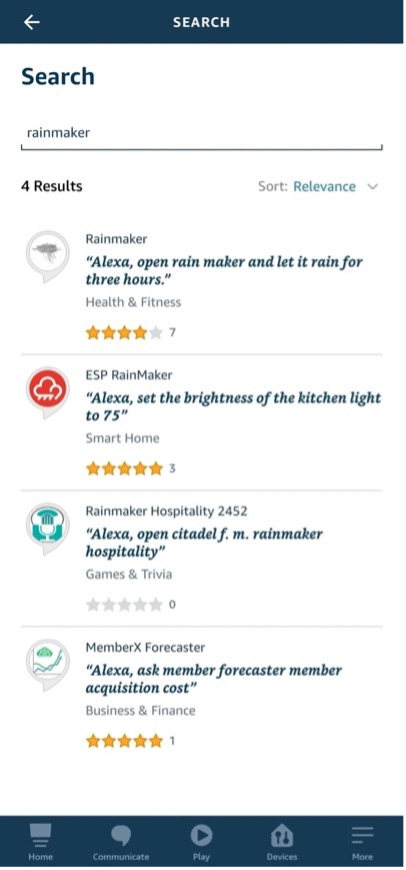
\includegraphics[height=1.3\textwidth,frame]{D9Z/9-14a} 
    \end{subfigure}\hspace{1em}
    \begin{subfigure}{0.4\textwidth}
        \RaggedRight
        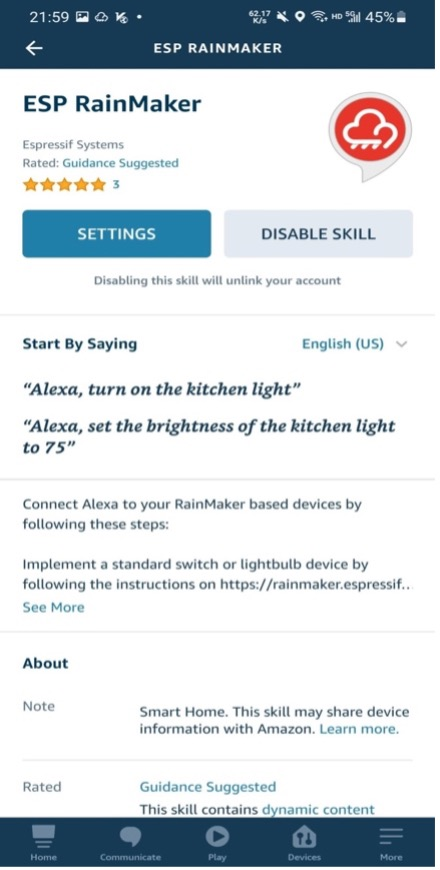
\includegraphics[height=1.3\textwidth,frame]{D9Z/9-14b}
    \end{subfigure}
    \caption{ESP RainMaker devices in Alexa}
\end{figure}

Figure 9.15 displays the ESP RainMaker devices in the Google Home. They can be controlled using voice commands such as “Hey Google, please turn off the light”.

\begin{figure}[h!]
    \Centering
    \begin{subfigure}{0.4\textwidth}
        \RaggedLeft
        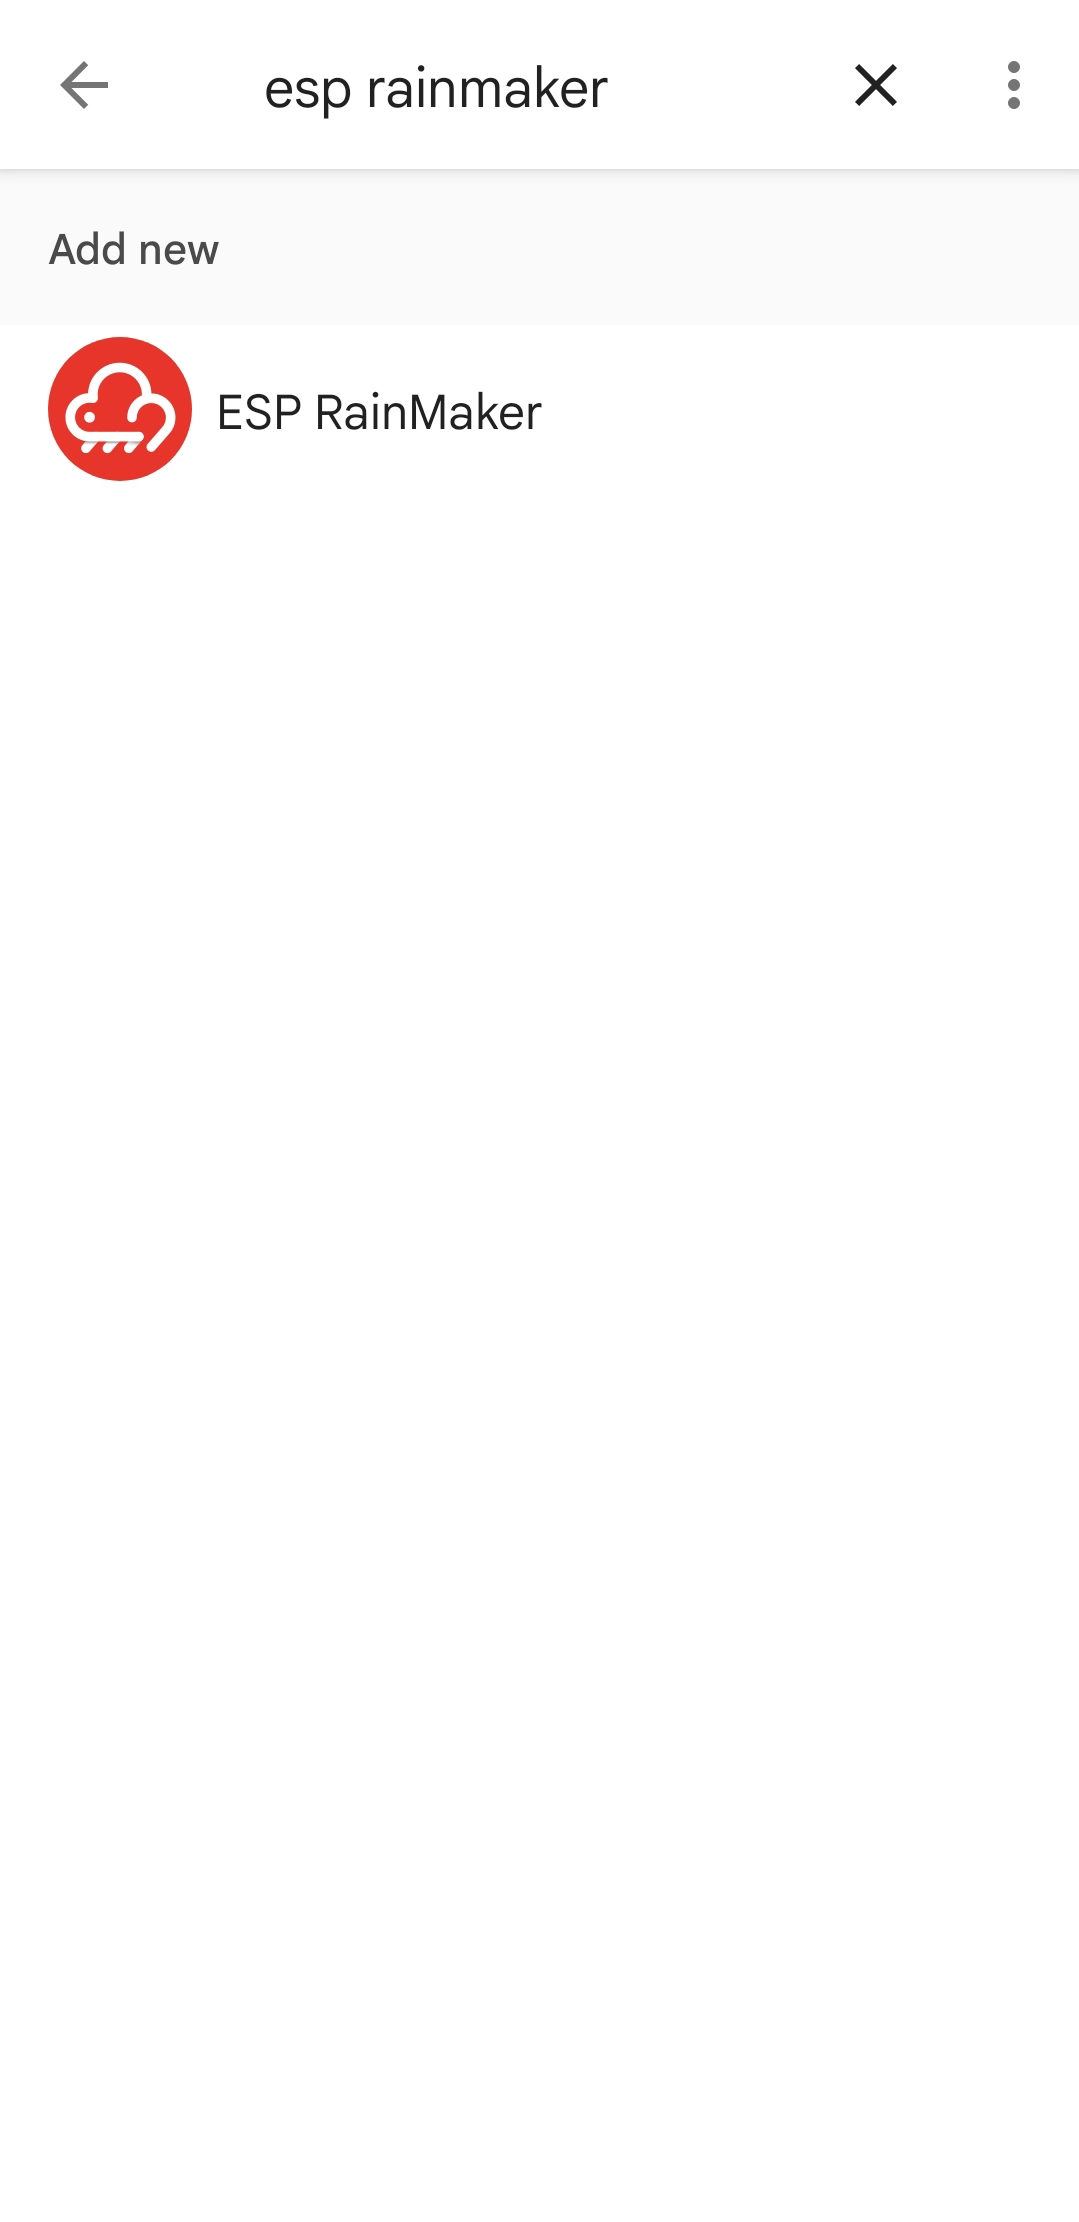
\includegraphics[height=1.3\textwidth,frame]{D9Z/9-15a} 
    \end{subfigure}\hspace{1em}
    \begin{subfigure}{0.4\textwidth}
        \RaggedRight
        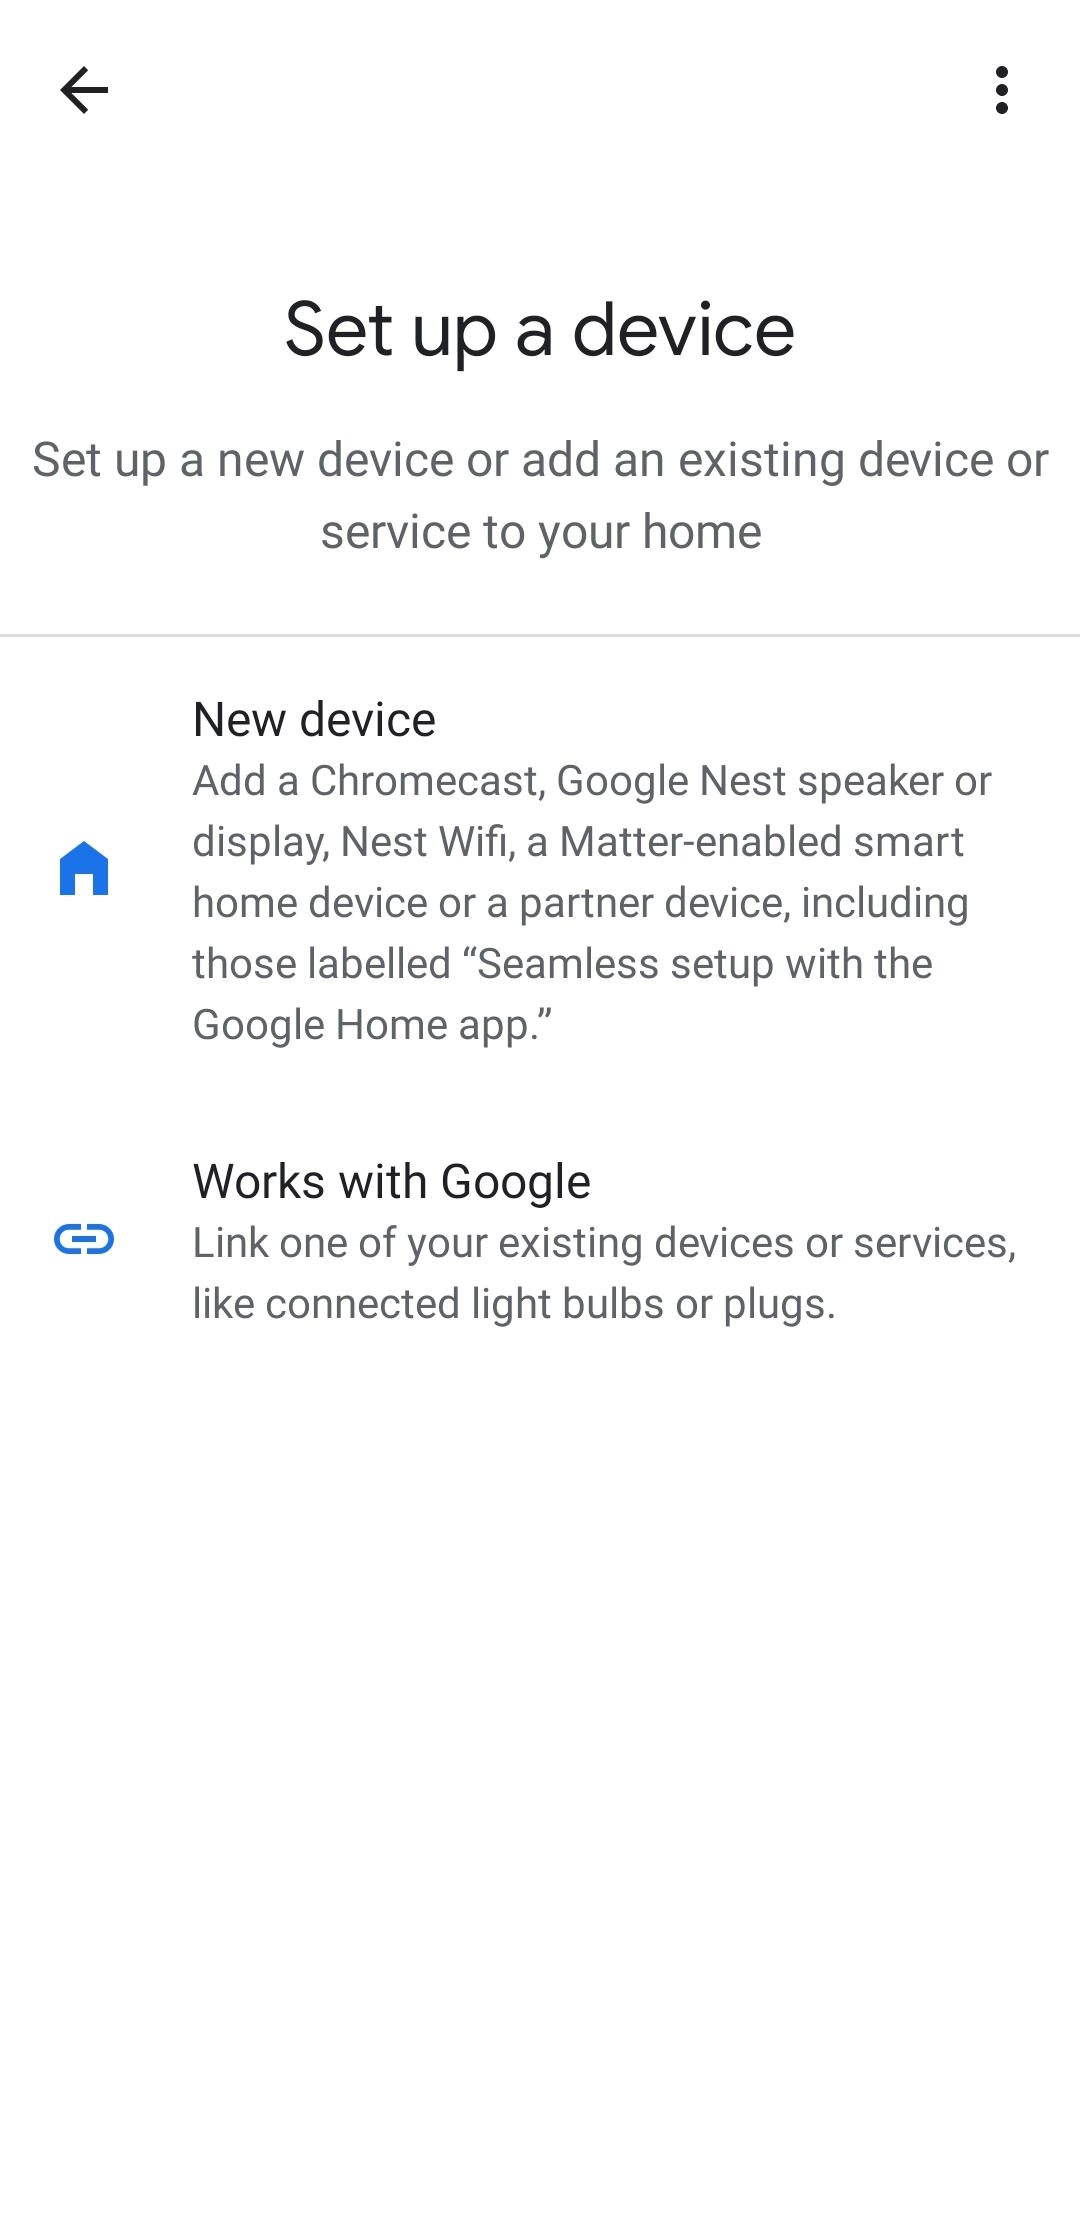
\includegraphics[height=1.3\textwidth,frame]{D9Z/9-15b}
    \end{subfigure}
    \caption{ESP RainMaker devices in Google Home}
\end{figure}

ESP RainMaker builds an intermediate layer in the cloud backend. This layer maps the standard parameter types and device types that are built into firmware to the formats that Alexa Skill and Google Assistant can understand. Therefore, device types in ESP RainMaker, such as smart lights and switches, are mapped to similar device types in Alexa Skill and Google Assistant, and their parameters, such as switch, brightness, and color, are mapped to corresponding capabilities and traits. If you only set brightness, you will get a smart light with adjustable brightness in Alexa and Google Home. If you also include color and CCT, you can adjust its color and color temperature.

\section{Summary}
In this chapter, we introduced remote control and the MQTT protocol. It is a commonly used protocol in remote control and connection of IoT devices to the cloud. It is now adopted by many mainstream cloud platforms, such as Amazon Cloud, Alibaba Cloud, Baidu Cloud, Tencent Cloud, and ESP RainMaker introduced in this chapter. This simple and lightweight protocol provides reliable network services for IoT devices in low-bandwidth and unstable network environments. 

Besides, we also covered how to build an MQTT broker locally to simulate the cloud platform, and how to generate server and client certificates for the TLS protocol handshake to ensure data security.

In the practice in this chapter, we took the development of a smart light product as an example to complete the remote control of devices using the ESP RainMaker platform over MQTT. Self Claiming is used to obtain certificates. Multiple sets of MQTT topics are used for device control, user-node mapping, and device status. The built-in basic services can perform the scheduling operation and OTA upgrade. With the completed cloud connection function of ESP RainMaker, smart lights can quickly be given voice control capabilities.

ESP RainMaker’s capabilities are not limited to this. Data collection and analysis, device-to-device linkage, and third-party scene triggers are all interesting functions yet not mentioned in this chapter. With these cloud functions, we can roughly calculate power consumption by counting the online/offline time and frequency of smart lights and found out how they work together with other hardware. These functions can be achieved using the open RESTful API. Chapter 10 will introduce the use of the RESTful API and use them to develop a smartphone app.
\end{document}